\documentclass[12pt]{article}

%Adapted from Adapted from UWA Engineering Final Year Project.


\usepackage[utf8]{inputenc}
\usepackage[x11names,dvipsnames,svgnames,table]{xcolor}

% general incantations
\usepackage[export]{adjustbox}
\usepackage{afterpage}
\usepackage{indentfirst}
\usepackage{graphicx}
\usepackage{placeins}
\usepackage{pdfpages}
\usepackage{algorithm2e}
\usepackage{array}
\usepackage{booktabs}
\usepackage[most]{tcolorbox}
\usepackage{calligra}
\usepackage{caption}
\usepackage{datetime}
\usepackage{dblfnote}
\usepackage{dirtytalk}
\usepackage{dsfont}
\usepackage{etex}
\usepackage{fancyhdr}
\usepackage{fix-cm}
\usepackage[T1]{fontenc}
\usepackage{textcomp,gensymb} %for \degree C symbol
\usepackage{lipsum}
\usepackage{listings}
\usepackage{transparent}
\usepackage[everyline=true,framemethod=tikz]{mdframed}
\usepackage{mparhack}
\usepackage{multicol}
\usepackage{multirow}
\usepackage{parskip}
\usepackage{lscape}
\usepackage{pdflscape}
\usepackage{pdfpages}
\usepackage{placeins}
\usepackage[document]{ragged2e}
\usepackage{rotating}
\usepackage{setspace}
\usepackage{subcaption}
\usepackage{threeparttable}
\usepackage[normalem]{ulem}
\usepackage{verbatim}
\usepackage{float}
\usepackage{soul} %highlighting, strike through etc.

%Automated appendices
\usepackage[titletoc,title,header]{appendix} %advanced functionality

%language settings
\usepackage[utf8]{inputenc}
\usepackage[portuguese]{babel}
\usepackage{csquotes}

%page setup
%this where we adjust the binding offset, if relevant
\usepackage[a4paper]{geometry}
\usepackage{lastpage} % for page 1 of n footers

%cross referencing
\usepackage[hidelinks]{hyperref}
\usepackage{cleveref}

%maths stuff
\usepackage{amsmath}
\usepackage{mathtools}

\setcounter{secnumdepth}{5}

%lists
\usepackage{enumitem}

%working collaboratively
\usepackage[backgroundcolor=yellow]{todonotes}

% bibliography file using harvard
\usepackage[style=ieee,backend=biber]{biblatex}
\bibliography{bibliography.bib} % with extension

%glossary for acronyms
\usepackage[acronym,nonumberlist,toc,section=subsection,numberedsection=nolabel]{glossaries} 
\makeglossaries

%line spacing
\linespread{1.25}

\lstdefinelanguage{docker}{
  keywords={FROM, RUN, COPY, ADD, ENTRYPOINT, CMD,  ENV, ARG, WORKDIR, EXPOSE, LABEL, USER, VOLUME, STOPSIGNAL, ONBUILD, MAINTAINER},
  keywordstyle=\color{blue}\bfseries,
  identifierstyle=\color{black},
  sensitive=false,
  comment=[l]{\#},
  commentstyle=\color{purple}\ttfamily,
  stringstyle=\color{red}\ttfamily,
  morestring=[b]',
  morestring=[b]"
}

\lstdefinelanguage{docker-compose}{
  keywords={image, environment, ports, container_name, ports, volumes, links},
  keywordstyle=\color{blue}\bfseries,
  identifierstyle=\color{black},
  sensitive=false,
  comment=[l]{\#},
  commentstyle=\color{purple}\ttfamily,
  stringstyle=\color{red}\ttfamily,
  morestring=[b]',
  morestring=[b]"
}
\lstdefinelanguage{docker-compose-2}{
  keywords={version, volumes, services},
  keywordstyle=\color{blue}\bfseries,
  keywords=[2]{image, environment, ports, container_name, ports, links, build},
  keywordstyle=[2]\color{olive}\bfseries,
  identifierstyle=\color{black},
  sensitive=false,
  comment=[l]{\#},
  commentstyle=\color{purple}\ttfamily,
  stringstyle=\color{red}\ttfamily,
  morestring=[b]',
  morestring=[b]"
}

\lstset{basicstyle=\small\ttfamily,
  showstringspaces=false,
  commentstyle=\color{red},
  keywordstyle=\color{blue},
  inputencoding=utf8,
  extendedchars=true
}

\begin{document}

\thispagestyle{empty}
\setlength\headheight{0pt} 
\begin{center}

\begin{center}

\includegraphics[width=0.45\linewidth]{img/um_logo.jpg}            
\end{center}	

        \vspace{0.25cm}
        {\scshape\LARGE Universidade do Minho \par}
        \vspace{0.25cm}
        {\scshape\Large Mestrado integrado em Engenharia Informática\par}
        \vspace{0.5cm}

        {\Large\bfseries Trabalho Prático\par}
        
        
        \vspace{0.5cm}
        {\Large\itshape Grupo 5\par}
        {\Large\itshape Diogo Pinto Ribeiro, A84442\par}
        {\Large\itshape João Nuno Cardoso Gonçalves de Abreu, A84802\par}
        {\Large\itshape José Diogo Xavier Monteiro, A83638 \par}
        {\Large\itshape Vasco António Lopes Ramos, PG42852\par}
        \vspace{0.25cm}

\vspace{0.7cm}
%Supervised by\par
Infraestrutura de Centro de Dados \\
4º Ano, 1º Semestre \\
Departmento de Informática\par
\vspace{0.7cm}
\large
\today

\end{center}

\clearpage
\restoregeometry
\justify

\pagenumbering{gobble}
%\input{sections/declaration}
%\section*{Acknowledgements}
Aqui é onde se agradece.
\pagebreak
%\section{Abstract} \label{section:abstract}
With the growing concern for the environment, the market of electric vehicles has great potential to reduce the CO2 emissions of transporting industry. With that in mind, this document addresses the adoption of electric vehicles (EVs) as a means of personal transport, in order to replace the internal combustion vehicles (ICVs) to reduce pollution emission and promote a cleaner and more healthier environment.

This document discusses previous work on this field and purposes a system dynamics model to better understand the current and future growth of this market and what factors influence it the most.

This study approaches a series of possible factors such as \textbf{driving range}, \textbf{price difference} between EVs and ICVs, \textbf{charging time}, among others and analyses how each of these factors can impact the market and in what scale/importance.

From the scenario and simulation results, it is possible to conclude that:
\begin{itemize}
\item A high density recharge infrastructure is essential to promote market's adoption;
\item Government subsidies are the major promoter of the electric vehicle industry adoption and evolution, especially in the early stages of this market;
\item Charging prices and electric vehicle price difference compared to ICVs are today's primary factor that customers consider when thinking of purchasing an EV;
\item Further development on the underlying batteries technology with the goal to improve performance and reduce charging time is an important necessity, since it can be a major reason to increase the electric vehicles adoption rate.
\end{itemize}

These conclusions agree on what most recent work in this field has been achieving and are also an interesting contact point with the work developed by Pedro Ferreira \cite{pedro-report}.

All the work related with this study can be found at \url{https://github.com/vascoalramos/ev-adoption-model}.

\clearpage

%List of figures and tables, automatic from thesis.
\pagenumbering{roman}
%Change ToC title
\renewcommand{\contentsname}{Índice}
\tableofcontents
\pagebreak

\listoffigures
\pagebreak
 
\listoftables
\pagebreak




\pagenumbering{arabic}

\setlength{\parindent}{5ex}
\section{Introdução}

Cada vez mais o ser humano encontra-se conectado e dependente da tecnologia, sendo que esta tem de ser capaz de se adaptar e responder com sucesso às necessidades exigentes de qualquer tipo de cliente. Para isso, possuir uma infraestrutura segura e confiável capaz de garantir o fluxo de informação sem erros e em tempo útil é essencial para um serviço de qualidade. Sendo assim, é fundamental que as infraestruturas estejam preparadas para responder a desafios relativos à tolerância a falhas, escalabilidade, alocação de recursos lidando com grandes volumes de dados, elevada disponibilidade, eficiência energética, entre outros.

Nesse sentido, este trabalho tem como objectivo não só consolidar os conhecimentos obtidos na unidade curricular Infraestruturas de Centro de Dados, nomeadamente no planeamento, configuração, análise de desempenho e operação de infraestruturas de elevada disponibilidade e desempenho, como também implementar um serviço escalável e de elevada disponibilidade de infraestruturas computacionais para a plataforma \textit{Wiki.js}. 

Ao longo dos próximos capítulos será apresentada a abordagem feita pelo grupo para cumprir com os requisitos acima descritos.
\pagebreak
\section{Arquitetura e Componentes do Wiki.js}

O projeto, que nos foi apresentado, consiste no planeio e operacionalização da instalação de uma plataforma \textbf{Wiki.js}, tal como toda a manutenção necessária ao seu bom funcionamento. Para esse efeito, começamos por desenvolver a arquitetura que servirá como base de todo o trabalho.

A aplicação \textbf{Wiki.js} encontra-se dividida entre \textit{frontend}, que apresentará a interface ao \textit{web client}, e \textit{backend} e utilizará uma base de dados para o armazenamento de dados:

\begin{figure}[h]
    \centering
    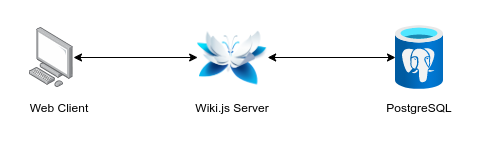
\includegraphics[width=\linewidth]{img/wiki_basic_arch.png}
    \caption{Diagrama da arquitetura do sistema}
    \label{fig_1}
\end{figure}

\subsection{Servidor Wiki.js}

\textbf{Wiki.js} é uma aplicação \textit{open source}, escrita em JavaScript e que corre em Node.js, oferecendo a funcionalidade de gerar páginas wiki completamente customizáveis e modulares.

Para além de ser uma aplicação web extremamente rápida e ter um design simplista e elegante, possui um vasto conjunto de ferramentas \textit{dev friendly} e oferece suporte para a base de dados \textbf{PostgreSQL} \cite{wiki-article}.

Numa primeira intalação (simplificada), esta plataforma, ficará instalada num servidor individual (servidor aplicacional). Aquando da comunicação pelos utilizadores, \textit{web clients}, terá de fornecer o \textit{frontend} ou camada de apresentação. Para além disso, o \textit{backend} irá comunicar com o servidor de base de dados, onde será armazenada toda a informação.

\subsection{Servidor PostgreSQL}

Tal como referido previamente, o nosso servidor aplicacional comunica (escrita e leitura de dados) diretamente com uma base de dados \textbf{PostgreSQL}, que estará instalada no seu próprio servidor.

Decidimos recorrer a este sistema de gestão de base de dados por vários motivos. Primeiramente, a própria documentação da plataforma \textbf{Wiki.js} recomenda o seu uso, \cite{wiki-requirements}. Depois, é o sistema mais popular do mercado e ganhou a sua extensa reputação devido à sua arquitetura, confiabilidade, integridade de dados, vasta gama de \textit{features} e dedicação à comunidade \textit{open source}. Além disso, está presente em todos os maiores sistemas operativos \cite{postgres-about}. Por fim, achamos que o facto de já estarmos acostumados à sua utilização, se mostraria uma mais valia na realização deste projeto.

\pagebreak
\section{Arquitetura Inicial}

De forma a perceber-se qual o comportamento do sistema como um todo, sem qualquer tipo de replicação ou otimização, decidiu-se fazer uma primeira instalação distribuída básica, utilizando \textit{Docker} e \textit{Docker Compose}, tendo por a configuração disponível na documentação do \textit{Wiki.js}, em \cite{wiki-docker}.

O objetivo desta instalação é conseguir avaliar o desempenho do sistema através da execução de um \textit{workload} com múltiplos testes de carga e, com base nos respetivos resultados, identificar e explorar os potenciais pontos críticos onde o sistema pode falhar ou perder desempenho.

Para tal, usou-se uma configuração de \textit{Docker Compose} com dois serviços (\textbf{\textit{db}} e \textbf{\textit{wiki}}), tal como se pode ver no anexo \ref{appendix:wiki-docker-compose}.

\subsection{Pontos Críticos do Sistema}

Para que seja possível garantir que um serviço possua uma elevada disponibilidade mantendo-se com um bom desempenho no atendimento de pedidos, torna-se necessário perceber quais são os \textbf{pontos críticos de falha e desempenho} do nosso sistema.

O principal cenário em que um sistema pode falhar é aquele em que um dos componentes que o constitui (ou mais) falhar, não existindo mais do que uma instância de cada um destes elementos. Isto pode acontecer quer por falhas de software/hardware, quer por falhas de energia. No nosso caso em concreto, com a nossa arquitetura inicial, possuímos 2 elementos: a \textbf{Base de Dados} e o servidor \textbf{Wiki.js}. Estes elementos não possuem qualquer réplica, o que significa que na eventualidade de um ou mais falhar, todo o sistema irá ficar inoperacional.

Outro dos principais pontos de falha e desempenho de uma aplicação são os \textbf{\textit{bottlenecks}}. Os \textit{bottlenecks} são situações em que um componente da aplicação limita todas as outras, diminuindo a performance do sistema. No nosso caso, o principal \textit{bottleneck} que identificámos é a \textbf{Base de Dados} visto que tanto serve pedidos do \textit{frontend} como do \textit{backend}. Dado que a nossa base de dados não está preparada com mecanismos de alta disponibilidade, prevemos que esta poderá a vir ser um ponto crítico do sistema.

Com estes pontos, ficámos com uma melhor noção do que poderá vir a ser um problema no nosso sistema, e quais serão algumas das soluções possíveis.

\subsection{Testes de Carga}

De modo a avaliar o desempenho da nossa instalação recorremos a \textbf{Testes de Carga} utilizando o \textbf{JMeter}. Utilizando GUI do \textit{JMeter} criámos 4 Testes que tentam simular um pouco do que será o funcionamento de uma \textit{Wiki} de um determinado produto ou serviço. Considerámos que no nosso cenário de teste utilizadores normais apenas consultam páginas enquanto que administradores têm a possibilidade de efetuar login e adicionar, editar ou remover páginas. Efetuámos essa segregação devido à diferença nos números de utilizadores e administradores, sendo os primeiros em número consideravelmente superior.

Os testes foram corridos no ambiente de linha de comandos de modo a poupar recursos das nossas máquinas, sendo que as limitações de hardware e as limitações relativas à \textbf{JVM} foram os principais obstáculos ao aumento da carga.

\subsubsection{Teste 1}

O Teste 1 visa representar o cenário mais básico: um utilizador aceder à página inicial da wiki. Para este teste irão ser utilizadas mais \textit{threads} do que nos restantes dado que num cenário real, o acesso à página inicial da wiki é o mais comum. Ao correr este teste é testado o seguinte método:

\begin{enumerate}
  \item GET /
\end{enumerate}

O teste foi corrido com 100, 1000, 5000 e 10000 \textit{threads} (utilizadores), sendo que recorremos aos relatórios gerados pelo \textit{JMeter} para apresentar os seguintes resultados. 

\begin{table}[h!]
\centering
    \begin{tabular}{ |c|c|c|c|  }
        \hline
        \multicolumn{4}{|c|}{Página Inicial} \\
        \hline
         Threads & Erro & Tempo Resposta Médio (ms) & \textit{Throughput (Trans./s)}\\
        \hline
        100   & 0.00\%   & 4129.90  & 17.51\\
        1000  & 0.00\%   & 11572.32 & 47.10\\
        5000  & 47.20\%  & 23539.35 & 98.41\\
        10000 & 67.87\%  & 24610.09 & 157.72\\
        \hline
    \end{tabular}
    \caption{Instalação Simples - Sumário do Teste 1}
    \label{table:1}
\end{table}

\vspace{2cm}

Analisando os dados da tabela, podemos verificar que com 100 e com 1000 utilizadores não obtemos nenhuma percentagem de erro. Ao subir para um valor na casa dos 5000 já começámos a obter uma percentagem significativa de erros, sendo que com 10000 essa percentagem é ainda superior. Esta percentagem de erros permite-nos ter uma perceção do limite da disponibilidade da instalação atual da aplicação. 

Ao aumentar o número de threads, verificámos também o aumento do \textit{Throughput} da aplicação, bem como do tempo de resposta médio aos pedidos. Este último valor é aquele que nos preocupa mais acerca do teste dado que também pode ser encarado como um indicador de performance do sistema. Mesmo em casos em que todos os pedidos são atendidos, o tempo de resposta é bastante elevado, como por exemplo, no caso de 1000 \textit{threads}, em que precisámos em média de 11.6 segundos para abrir a página inicial, algo que é inaceitável nos padrões atuais. Os tempos de resposta elevados em conjunto com a elevada taxa de erro significam que o nosso sistema não está a responder corretamente aos pedidos efetuados. 

\begin{figure}[ht!]
    \centering
    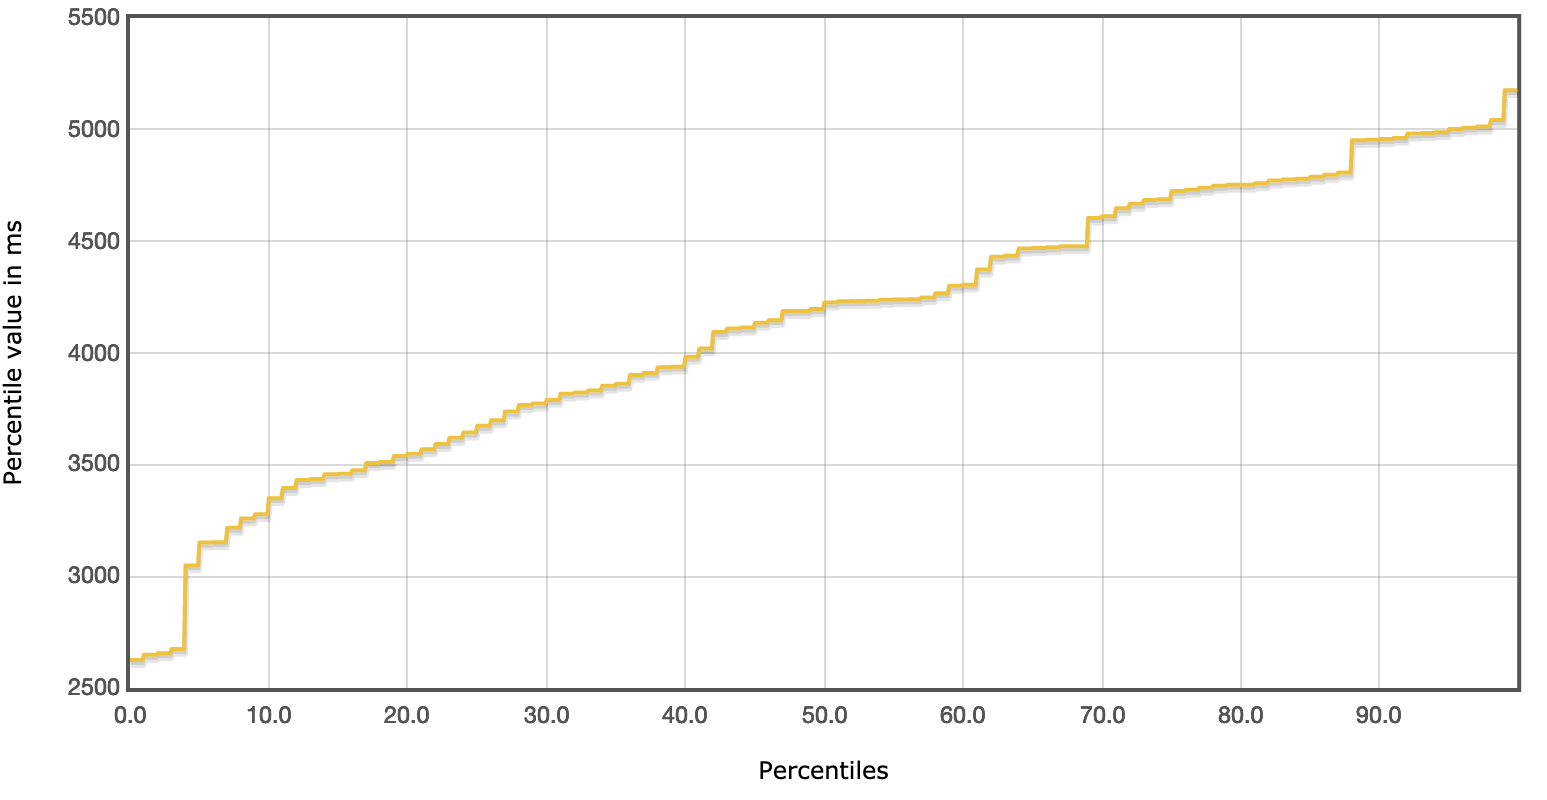
\includegraphics[width=.45\linewidth]{img/testes/i-t1-100.png}
    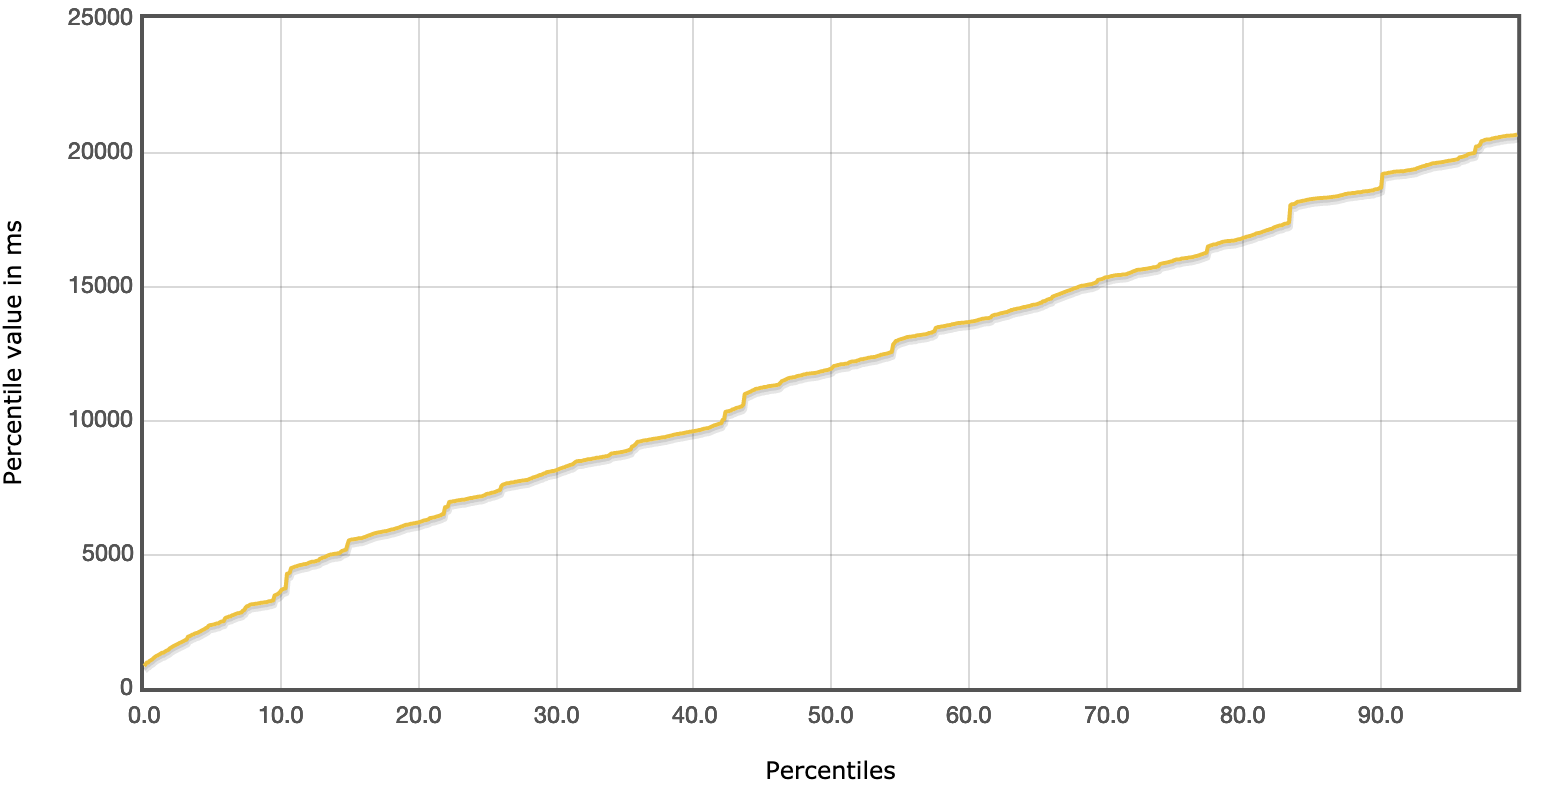
\includegraphics[width=.45\linewidth]{img/testes/i-t1-1000.png}
    \caption{Percentil Tempo de Resposta para 100 e 1000 Threads}
\end{figure}

\begin{figure}[ht!]
    \centering
    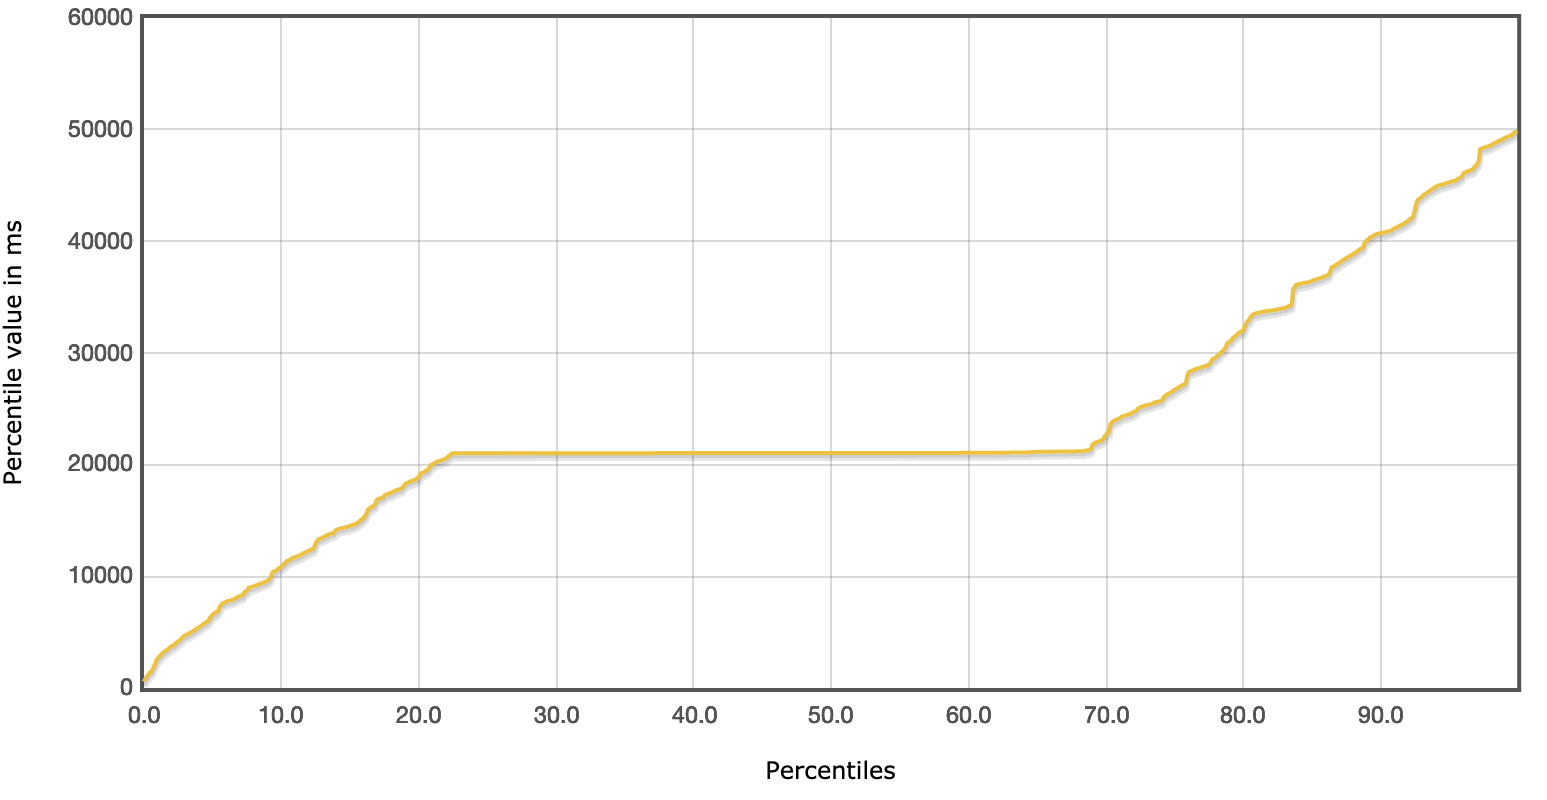
\includegraphics[width=.45\linewidth]{img/testes/i-t1-5000.png}
    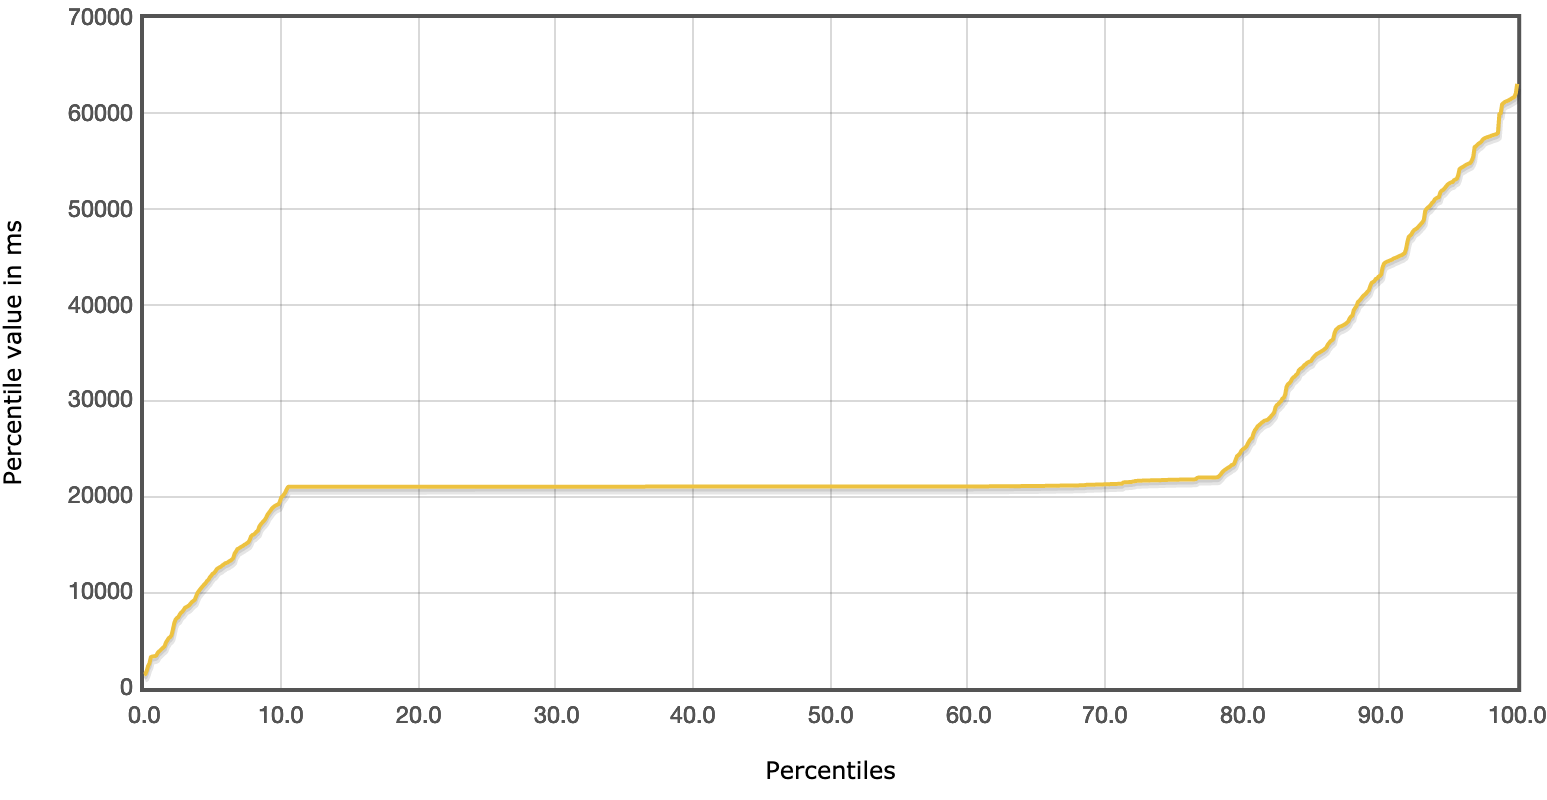
\includegraphics[width=.45\linewidth]{img/testes/i-t1-10000.png}
    \caption{Percentil Tempo de Resposta para 5000 e 10000 Threads}
\end{figure}

\vspace{2cm}
Verificando os gráficos apresentados, fica ainda mais evidente que os tempos de resposta da aplicação são bastante elevados.

\subsubsection{Teste 2}

O Teste 2 visa representar o cenário em que um utilizador entra na página inicial, navegando de seguida para uma outra página da wiki. Neste caso em específico, todas as \textit{threads} abrem a mesma página após pedirem a página inicial e esperarem 1000 milissegundos. Ao correr este teste são testados os seguintes métodos:

\begin{enumerate}
  \item GET /
  \item GET /en/ICD
\end{enumerate}

O teste foi corrido com 1000 e 5000 \textit{threads}, sendo que recorremos aos relatórios gerados pelo \textit{JMeter} para apresentar os seguintes resultados. Estes valores foram escolhidos pela sua relevância tendo em conta o teste anterior.

\begin{table}[h!]
\centering
    \begin{tabular}{ |c|c|c|c|c|  }
        \hline
        \multicolumn{4}{|c|}{Página Inicial} \\
        \hline
         Threads & Erro & Tempo Resposta Médio (ms) & \textit{Throughput (Trans./s)}\\
        \hline
        1000  & 0.00\%   & 9328.98  & 52.63\\
        5000  & 49.56\%  & 25202.86 & 109.55\\
        \hline
    \end{tabular}
    \caption{Instalação Simples - Sumário do Teste 2}
    \label{table:1}
\end{table}

Analisando os dados da tabela, podemos verificar que com 1000 utilizadores não obtemos nenhuma percentagem de erro. Quando aumentamos para valores na casa dos 5000 começámos a obter uma percentagem significativa de erros, que neste caso já se demonstra inaceitável para uma plataforma funcional. Esta percentagem de erros mostra-nos um pouco qual o limite da disponibilidade da aplicação de momento. 

Ao aumentar o número de threads, verificámos também o aumento do \textit{Throughput} da aplicação, bem como do tempo de resposta médio aos pedidos. Este último valor, dado que também serve de medida de performance do sistema, mostra-nos que nos casos em que assegurámos que todos os pedidos são atendidos, estes esperam uma quantidade de tempo considerável. 

\begin{figure}[ht!]
    \centering
    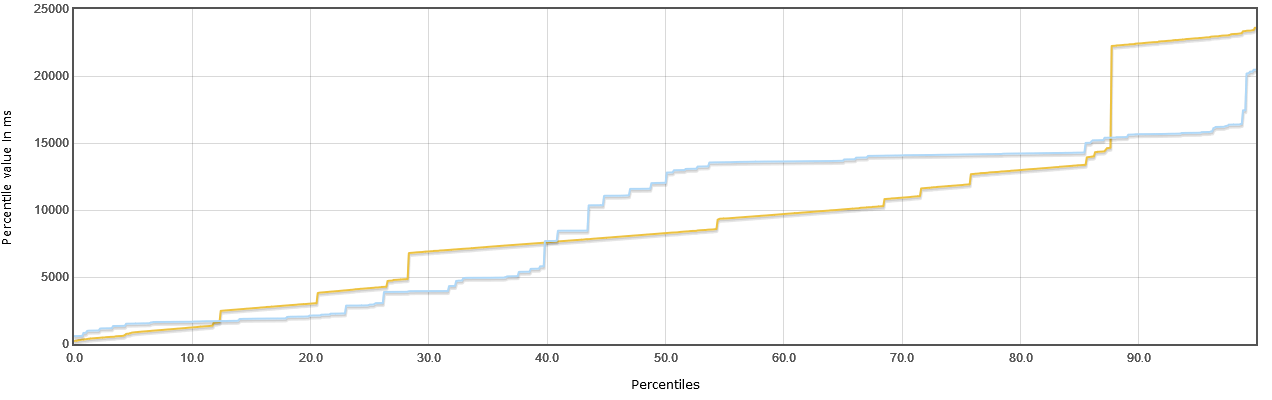
\includegraphics[width=.45\linewidth]{img/testes/i-t2-1000.png}
    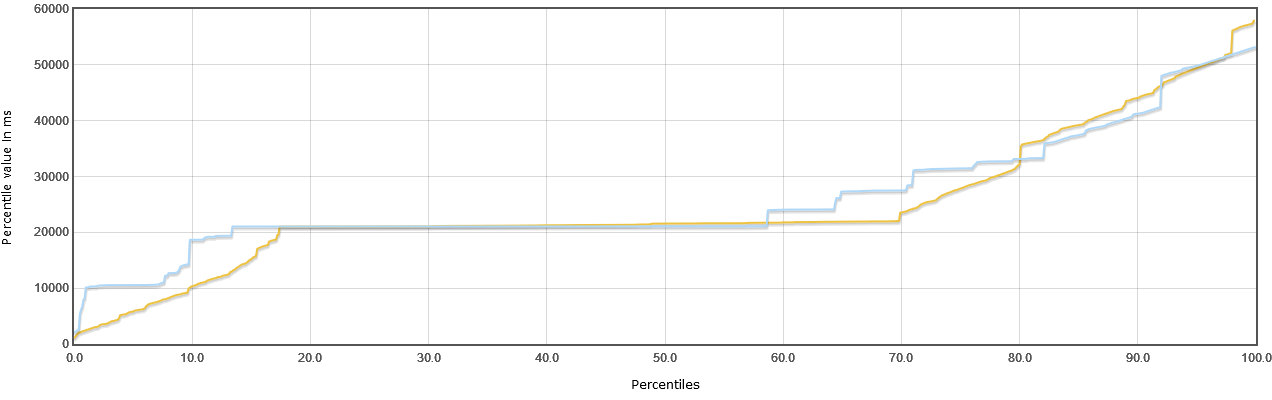
\includegraphics[width=.45\linewidth]{img/testes/i-t2-5000.png}
    \caption{Percentil Tempo de Resposta para 1000 e 5000 Threads}
\end{figure}

Verificando os gráficos apresentados, em que a linha azul representa os pedidos referentes à página de teste e a linha laranja os pedidos referentes à página inicial, fica ainda mais evidente que os tempos de resposta da aplicação são bastante elevados.

\subsubsection{Teste 3}

O Teste 3 visa representar o cenário em que um administrador efetua login no sistema, sendo redirecionado para a página principal. Ao correr este teste são testados os seguintes métodos:

\begin{enumerate}
  \item GET  /login
  \item POST /graphql
  \item GET  /
\end{enumerate}

O teste foi corrido com 100, 250, 500, 1000 e 5000 \textit{threads}, sendo que recorremos aos relatórios gerados pelo JMeter para apresentar os seguintes resultados.
O processo de login é constituido pelos 3 pedidos apresentados, sendo que o conteúdo do POST que é feito possui o endereço de email e a password da conta utilizada no teste. Estes 3 pedidos foram encapsulados num processo mais generalizado que representa o login como um todo. Optámos por esta visão de modo a representar de modo mais fidedigno o ato de efetuar login, dado que não é possível efetuar login se uma das operações falhar. Outra atenção que tivemos, foi o cancelamento de uma \textit{thread} no caso de um dos pedidos falhar.

\begin{table}[h!]
\centering
    \begin{tabular}{ |c|c|c|c|c|  }
        \hline
        \multicolumn{4}{|c|}{Página Inicial} \\
        \hline
         Threads & Erro & Tempo Resposta Médio (ms) & \textit{Throughput (Trans./s)}\\
        \hline
        100   & 0.00\%   & 6205.00  & 14.13\\
        250   & 0.00\%   & 7104.55  & 28.19\\
        500   & 0.00\%   & 16982.52 & 25.65\\
        1000  & 1.09\%   & 30312.79 & 22.80\\
        5000  & 64.74\%  & 90830.34 & 25.57\\
        \hline
    \end{tabular}
    \caption{Instalação Simples - Sumário do Teste 3}
    \label{table:1}
\end{table}

Analisando os dados da tabela, podemos verificar que com 100, 250 e 500 não obtemos nenhuma percentagem de erro. Ao subir para valor na casa dos 1000 já começámos a obter uma percentagem de erros, embora insignificativa. Nos 5000 utilizadores, a maioria deles já não consegue efetuar login. Esta percentagem de erros mostra-nos um pouco qual o limite da disponibilidade da aplicação de momento. 

Ao aumentar o número de threads, verificámos também o aumento do \textit{Throughput} da aplicação até um certo ponto, sendo que estagnou um pouco ao chegar às 500 threads. O tempo de resposta médio aos pedidos por sua vez não estagnou, subindo para valores elevados, mesmo sem a ocorrência de erros.

Nos gráficos apresentados, as \textbf{linhas vermelhas} representam o pedido \textbf{GET /login}, as \textbf{linhas azuis} representam o pedido \textbf{POST /graphql}, as \textbf{linhas amarelas} representam o pedido \textbf{GET /} e as \textbf{linhas verdes} representam o \textbf{Login} como um todo. Através destes gráficos, fica ainda mais evidente que os tempos de resposta da aplicação são bastante elevados.



\begin{figure}[ht!]
    \centering
    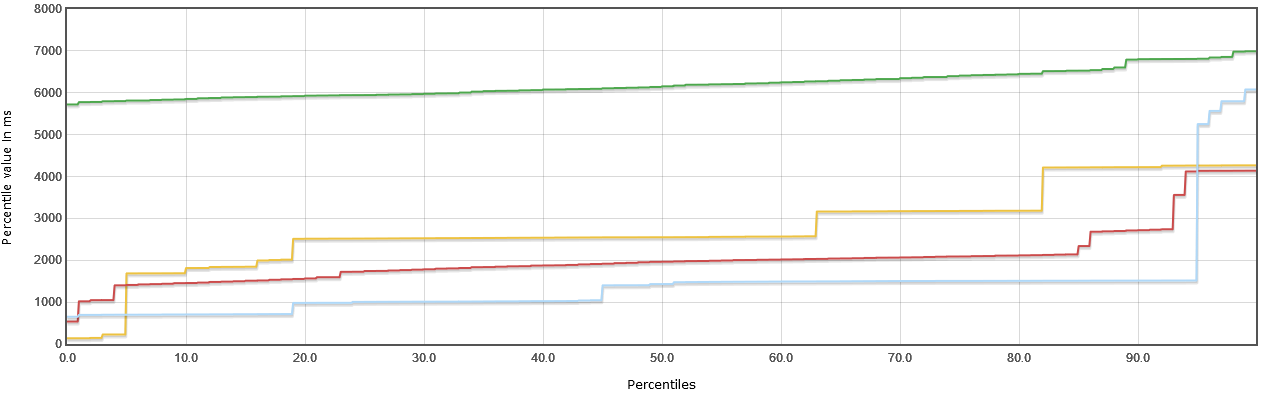
\includegraphics[width=.45\linewidth]{img/testes/i-t3-100.png}
    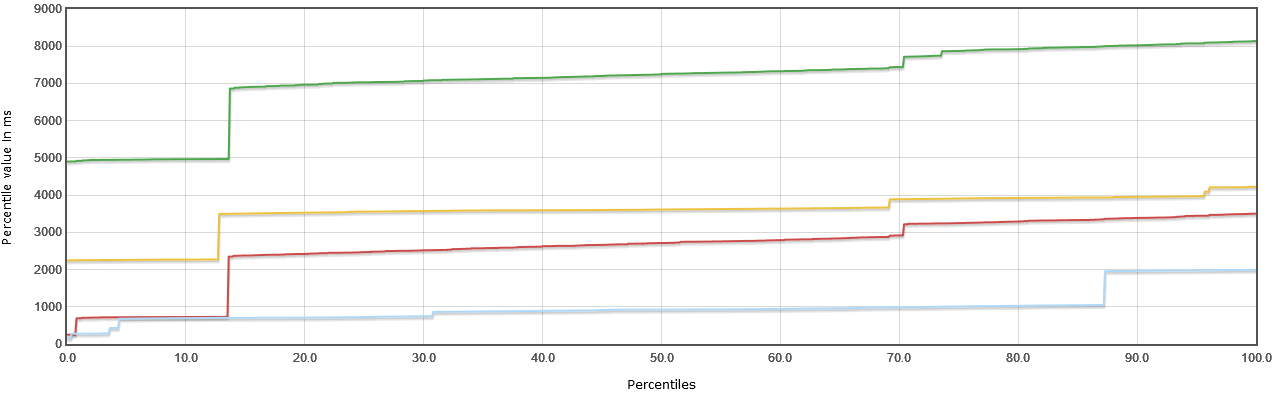
\includegraphics[width=.45\linewidth]{img/testes/i-t3-250.png}
    \caption{Percentil Tempo de Resposta para 100 e 250 Threads}
\end{figure}

\begin{figure}[ht!]
    \centering
    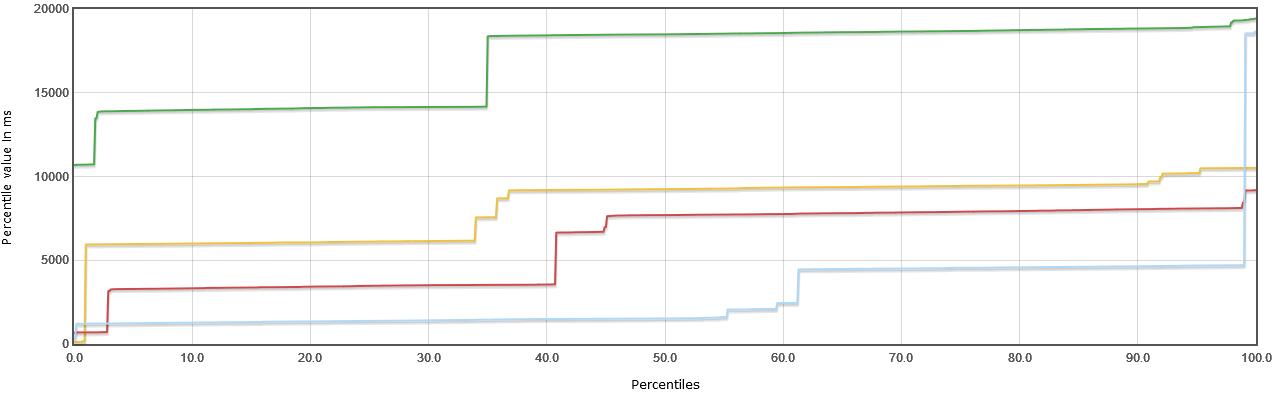
\includegraphics[width=.45\linewidth]{img/testes/i-t3-500.png}
    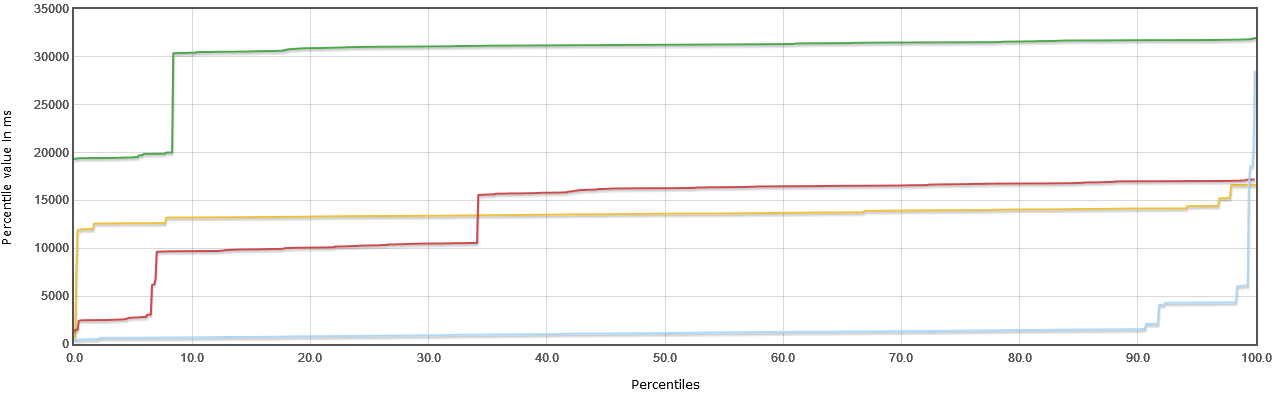
\includegraphics[width=.45\linewidth]{img/testes/i-t3-1000.png}
    \caption{Percentil Tempo de Resposta para 500 e 1000 Threads}
\end{figure}

\begin{figure}[ht!]
    \centering
    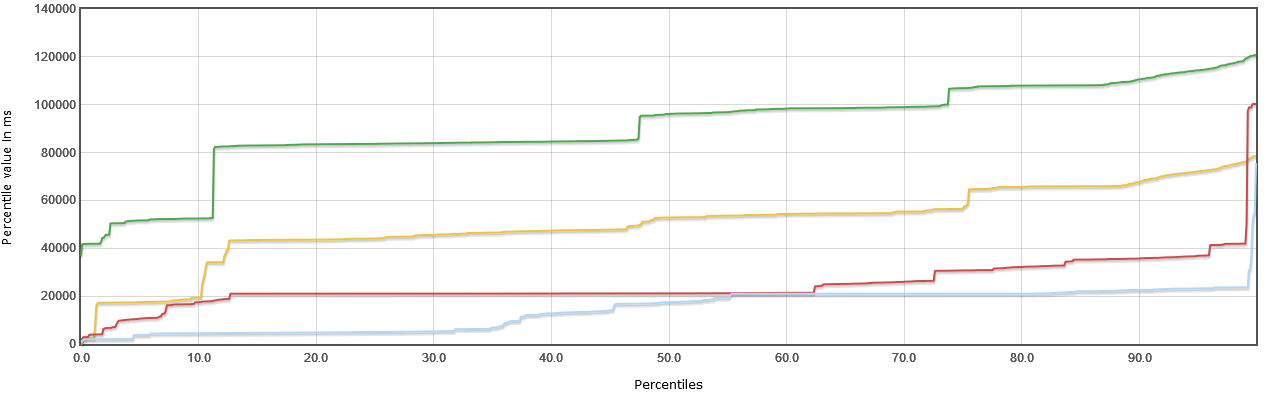
\includegraphics[width=.9\linewidth]{img/testes/i-t3-5000.png}
    \caption{Percentil Tempo de Resposta para 5000 Threads}
\end{figure}

% Para não haver texto a ir para espaços entre imagens
\pagebreak

\subsubsection{Teste 4}

O Teste 4 visa representar o cenário em que um administrador efetua login no sistema, sendo redireccionado para a página principal, seguido da criação de uma nova página wiki. Ao correr este teste são testados os seguintes métodos:

\begin{enumerate}
    \item GET /login
    \item POST /graphql
    \item GET /
    \item GET /e/en/ThreadNum-Pagename
    \item POST /graphql
    \item GET /e/en/ThreadNum-Pagename
\end{enumerate}

Nos métodos podemos encontrar as palavras \textit{ThreadNum} e \textit{Pagename}, que na verdade são variáveis. Cada \textit{thread} onde corremos os testes terá um \textit{ThreadNum} único, de maneira a conseguirmos saber que páginas cada \textit{thread} criou, e optamos por dar o nome à página a data do momento em que é criada em milissegundos para sabermos quando e por que ordem foram criadas as novas páginas. Isto é possível tomando partido das funções \texttt{\_\_time()} e \texttt{\_\_threadNum} do \textit{JMeter}.

O teste foi corrido com 100, 250 e 500 \textit{threads}, sendo que recorremos aos relatórios gerados pelo \textit{JMeter} para apresentar os seguintes resultados. A única diferença entre este teste e o anterior é que agora criamos uma página nova depois de fazermos o login, enquanto que no outro o teste acabaria precisamente depois de realizarmos o login. O processo de criação duma nova página é constituído pelos 3 últimos pedidos apresentados, sendo que o conteúdo do POST possui o conteúdo que a nova página irá apresentar. Estes 3 pedidos foram encapsulados num processo mais generalizado que representa a criação duma nova página como um todo. Optámos por esta visão de modo a representar de modo mais fidedigno o ato de criar uma nova página, dado que não é possível criá-la se uma das operações falhar. Sendo assim, preferimos separar a operação de efetuar login da criação da nova página para podermos avaliar individualmente cada um dos processos. 

\begin{table}[H]
\centering
\begin{tabular}{|c|c|c|p{3.5cm}|p{3cm}|}
\hline
Threads              & Operação & Erro    & Tempo Resposta Médio (ms) & \textit{Throughput (Trans./s)} \\ \hline
\multirow{2}{*}{100} & Login    & 0.00\%  & 4686.52                   & 17.05                          \\
                     & New Page & 18.00\% & 244610.95                 & 0.40                           \\ \hline
\multirow{2}{*}{250} & Login    & 0.00\%  & 12209.70                  & 18.49                          \\
                     & New Page & 37.14\% & 369123.91                 & 0.46                           \\ \hline
\multirow{2}{*}{500} & Login    & 0.00\%  & 23461.58                  & 19.98                          \\
                     & New Page & 84.25\% & 345850.68                 & 1.30                           \\ \hline
\end{tabular}
\caption{Instalação Simples - Sumário do Teste 4}
\end{table}

Analisando os dados da tabela, podemos verificar que as operações de login não possuem qualquer erro, enquanto que as da criação de páginas apresentam sempre erros, aumentando com o número de \textit{threads}. Podemos dizer que os tempos de resposta também aumentam proporcionalmente com o número de \textit{threads} mas o \textit{throughput} fica estagnado, seja qual for a operação e também o número de \textit{threads}!

Nos gráficos apresentados, as linhas \textbf{vermelho-escuro, roxo e amarelo-escuro} são as mais visíveis e ao mesmo tempo preocupantes, representando o \textbf{login, New Page e GET Page}, respetivamente. 

\begin{figure}[ht!]
    \centering
    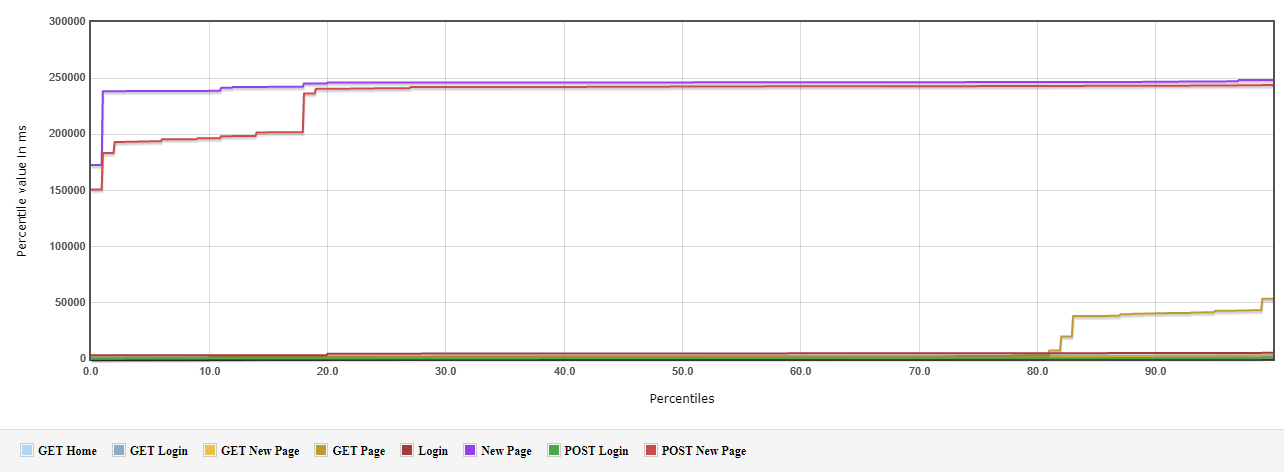
\includegraphics[width=.9\linewidth]{img/testes/i-t4-100.png}
    \caption{Percentil Tempo de Resposta para 100 Threads}
\end{figure}

\begin{figure}[ht!]
    \centering
    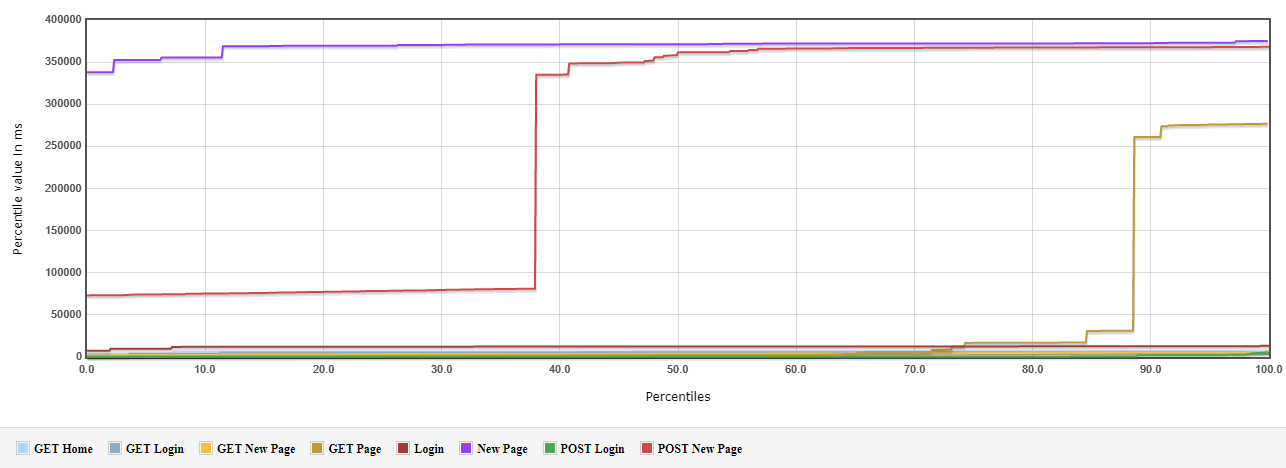
\includegraphics[width=.9\linewidth]{img/testes/i-t4-250.png}
    \caption{Percentil Tempo de Resposta para 250 Threads}
\end{figure}

\begin{figure}[ht!]
    \centering
    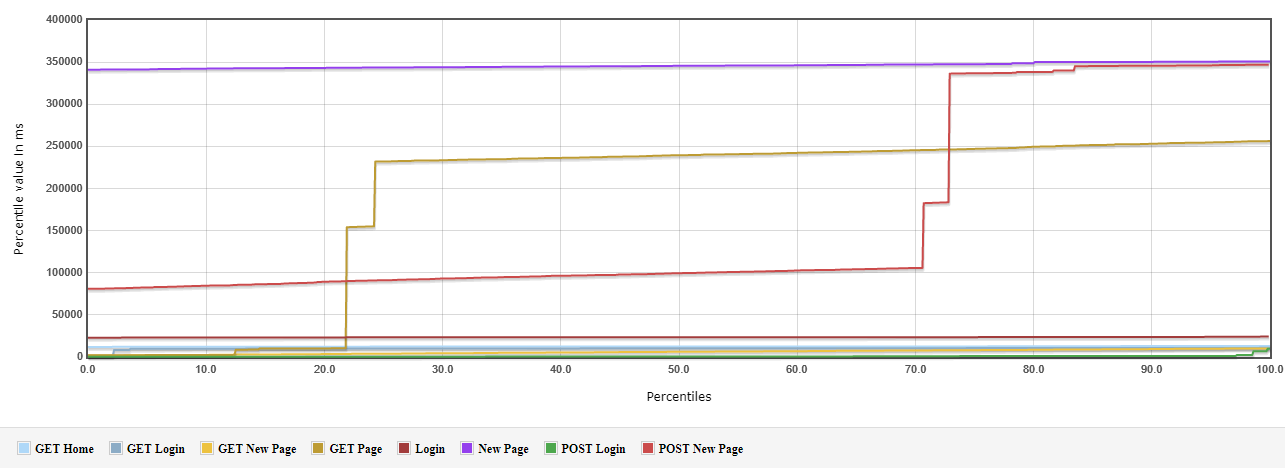
\includegraphics[width=.9\linewidth]{img/testes/i-t4-500.png}
    \caption{Percentil Tempo de Resposta para 500 Threads}
\end{figure}

\subsection{Análise de Desempenho}

Após analisarmos os resultados do \textbf{Testes de Carga} listados na secção anterior, somos agora capazes de efetuar uma análise face ao desempenho desta versão inicial.

A primeira conclusão a que chegámos é que apesar de um pedido ser atendido, não significa que o sistema esteja a operar de modo aceitável, isto é, possua tempos de resposta aceitáveis ou as respostas representem o estado esperado do sistema. Nos nossos testes, mesmo com percentagens de erro nulas, os tempos de resposta médios foram bastante elevados. Isto confirma a nossa suspeita acerca de \textbf{\textit{bottlenecks}} no nosso sistema.

Outra conclusão que tirámos prende-se nas percentagens de erro relativas a situações em que temos números de utilizadores mais elevados. Quando o número de utilizadores sobe, a nossa plataforma baixa consideravelmente a sua disponibilidade, chegando a ponto em que fica inoperacional.

As conclusões obtidas através dos testes de carga em conjunto com a possibilidade de um dos nossos elementos falhar, tal como visto na Secção 3.1, levam-nos a crer que a nossa implementação do Wiki.js é de \textbf{baixa disponibilidade} e possui uma \textbf{performance baixa}. Isto leva-nos à necessidade de implementar o Wiki.js num ambiente diferente, tal como iremos ver no capítulo a seguir.

\pagebreak
\section{Arquitetura Implementada}

Nesta Secção iremos descrever a arquitetura que implementámos para obter uma infraestrutura de elevada disponibilidade e desempenho, explicando quais as ferramentas utilizadas e explicando como estas resolvem os problemas identificados anteriormente. De modo a comparar a arquitetura implementada com a anterior, iremos efetuar os mesmos testes de carga de modo a comparar as duas soluções para poder efetuar comparações.

\subsection{Camada de Persistência}

Para a camada de persistência do sistema, iremos apresentar as componentes que a constituem pela ordem de implementação. 

A primeira componente desta camada consiste num grupo de VM's que constituem um \textbf{DRBD} (\textit{Distributed Replicated Block Device}) que são acedidas utilizando o protocolo \textbf{iSCSI} (\textit{Internet Small Computer Systems Interface}). Para esta componente criámos \textbf{duas instâncias de VM} na GCP com \textbf{2 vCPU} e \textbf{4GB de memória}. Cada uma das máquinas possui um disco \textbf{SSD de 20GB} onde foi instalado o sistema operativo (CentOS 8). A utilização de DRBD deve-se ao facto de este permitir garantir a replicação dos nossos dados. Para o armazenamento dos dados, cada uma das instâncias possui um \textbf{disco SSD de 50 GB} que irá ser atribuída a um recurso DRBD, sendo que o denominámos de \textbf{d1}. Ambas as instâncias foram sinalizadas como primárias para permitir que estas sejam utilizadas sem qualquer tipo de restrição. Para finalizar, numa das instâncias foi colocado um sistema de ficheiros no formato xfs, sendo estas alterações sincronizadas com a segunda instância. Após finalizada o setup do DRBD, avançámos para o setup do iSCSI \textit{target}.

A segunda componente desta camada consiste num grupo de VM's que constituem um cluster de elevada disponibilidade. Este cluster é constituído por \textbf{3 nodos}, tendo cada um \textbf{2 vCPU} e \textbf{8GB de memória}. Cada uma das máquinas possui um disco \textbf{SSD de 20GB} onde foi instalado o sistema operativo (CentOS 8). Cada uma das instâncias foi configurada com o cliente \textbf{iSCSI}, ligando-se a cada um dos \textit{targets}. Após esta configuração do iSCSI foi colocado um serviço \textbf{multipath}. De seguida foi feito o setup do \textbf{\textit{High-Availability Cluster}} da RedHat em cada uma das três instâncias, sendo este cluster composto por três nodos: \textbf{cluster1}, \textbf{cluster2} e \textbf{cluster3}. Neste cluster foram definidos dois serviços: o serviço \textbf{fs}, que consiste no sistema de ficheiros replicado anteriormente criado, e o serviço \textbf{bd}, que consiste na configuração da base de dados postgres que pretendemos manter.

A terceira e última componente que compõe a camada de persistência é um \textbf{\textit{(tcp) load balancer}} interno, que tem como principal função encaminhar os pedidos para o nó \textit{director} e, também, verificar se cada um dos nós do cluster se encontra operacional. Na eventualidade de o nó ativo ficar inoperacional, o \textit{load balancer} automaticamente comunica com o nó seguinte. Para conseguir isto agrupámos os nós do cluster em dois grupos: um grupo primário e um grupo secundário. O cluster1 foi adicionado ao grupo primário, sendo este o principal nodo do cluster. O cluster2 e o cluster3 foram adicionados ao grupo secundário, sendo que no caso do nodo principal falhar, o \textit{failover} é feito para um destes nodos. 

O acesso a esta camada de persistência é então feito a partir do \textit{load balancer}. Deste modo, possuímos uma camada de persistência que nos garante elevada disponibilidade bem como replicação do disco com os dados, isto é, no caso de um dos elementos que compõe esta camada falhar, o serviço não é interrompido, e no caso de um dos discos de armazenamento falhar, possuímos uma cópia de todos os dados, mantendo-se o serviço sem interrupções. Com a utilização de discos SSD somos capazes de implementar melhorias de \textit{performance}, tornando o nosso sistema mais rápido no geral.


\subsection{Camada Aplicacional}
A camada aplicacional tem a responsabilidade de tratar os pedidos e responder-lhes devidamente. Tal como se pode ver na figura \ref{fig:final-arch}, para esta camada decidiu-se ter três servidores semelhantes, cada um com a aplicação \textit{Wiki.js} instalada. Tanto para a camada aplicacional como para a camada web, decidiu-se ter VMs semelhantes com:

\pagebreak

\begin{itemize}
\item 2 CPUs;
\item 8 GB de Memória RAM;
\item 10 GB de disco;
\item Sistema operativo Ubuntu 20.04 LTS.
\end{itemize}

A razão para ter 3 servidores semelhantes na camada aplicacional serve o propósito de uma maior paralelização no atendimento de pedidos, o que de um modo geral permite diminuir os tempos de resposta, isto é, tornar as operações mais rápidas e distribuir a carga para várias instâncias da aplicação, ao invés de sobrecarregar uma única instância da aplicação.

A razão anterior foca-se no desempenho, outra razão tem que ver com elevada disponibilidade, pois, se um dos servidores entrar em falta e não for capaz de responder a pedidos, temos os outros dois servidores a responder. No limite, podem entrar em falta 2 dos 3 servidores aplicacionais. No caso dos 3 servidores falharem, o serviço fica indisponível.

Como nota final relativamente ao \textit{deployment} desta camada, para facilitar a manutenção das aplicações, em cada VM criou-se um serviço associado à aplicação, que foi utilizado para pôr as aplicações a correr e que facilita qualquer tipo de manutenção das mesmas através das premissas de \textit{enable}, \textit{disable}, \textit{start}, \textit{stop}, \textit{restart}, etc dos serviços \textit{Linux}. 

\subsection{Camada Web (\textit{Load Balancers})}
A camada mais superficial (mais próxima da \textit{Internet}) é a camada \textit{web}. Esta tem a responsabilidade de receber os pedidos e distribuí-los pelos vários servidores aplicacionais existentes (\textit{load balancer} e \textit{reverse proxy}), bem como controlar o tráfego, através de regras de \textit{firewall}.

Esta camada dividi-se em duas sub-camadas:
\begin{itemize}
\item Um load balancer externo que serve como ponto de acesso ao sistema (é o componente mais superficial de toda a estrutura) e distribui os pedidos pelos servidores \textit{web};
\item Um conjunto de 3 servidores \textit{web} que distribuem os pedidos pelos vários servidores aplicacionais.
\end{itemize}

Olhando primeiro para os servidores \textit{web}, em si, cada um destes corre uma instância de \textbf{\textit{NGINX}}, configurada para receber pedidos e distribuí-los pelos 3 servidores aplicacionais. Com o objetivo de melhorarmos o tipo de distribuição de carga decidimos usar a opção \textbf{\textit{least\_conn}} que o NGINX fornece e que distribui a carga pelos vários servidores aplicacionais tendo em conta o seu número de conexões ativas.

Novamente, a decisão de ter 3 servidores \textit{web} segue a mesma lógica dos servidores aplicacionais: por um lado, dar alto desempenho ao aumentar o número de servidores \textit{web}, ao invés de ter apenas um, diminuindo a carga que cada um recebe e, por outro lado, ter alto disponibilidade pois, o sistema permite que, no limite, falhem 2 dos 3 servidores \textit{web}, sem que o sistema fique comprometido e/ou indisponível.

De notar que, tanto nos servidores \textit{web} como nos servidores aplicacionais a infraestrutura escolhida permite remover o problema do \textit{Single Point of Failure} (SPOF).

Por fim, temos o \textit{load balancer} externo para servir como ponto único de acesso ao sistema pela Internet/\textit{Web}. Este \textit{load balancer} distribui os pedidos que recebe pelos 3 servidores \textit{web} e, apesar de trazer a vantagem de permitir um ponto único de acesso e de abstrair o utilizador final de toda a estrutura que está por trás do sistema, tem a desvantagem de que se este serviço falha, todo o sistema fica indisponível para os utilizadores. Tendo isto em conta e de forma a limitar esta desvantagem, utilizámos um serviço da \textit{Google Cloud Platform}: um \textit{HTTP External Load Balancer} que, segundo a própria \textit{GCP}, tem elevada disponibilidade e uma probabilidade de falha muito baixa. Este serviço permite, então, distribuir os pedidos que recebe pelas 3 instâncias do servidor \textit{web} e tem, também, \textit{healthchecks} de 30 em 30 segundos para os servidores \textit{web}, de forma a conseguir perceber quais deles é que estão disponíveis para receber pedidos e assim adaptar o seu \textit{routing} do tráfego.

\subsection{Representação Geral da Arquitetura}

\begin{figure}[h!]
    \centering
    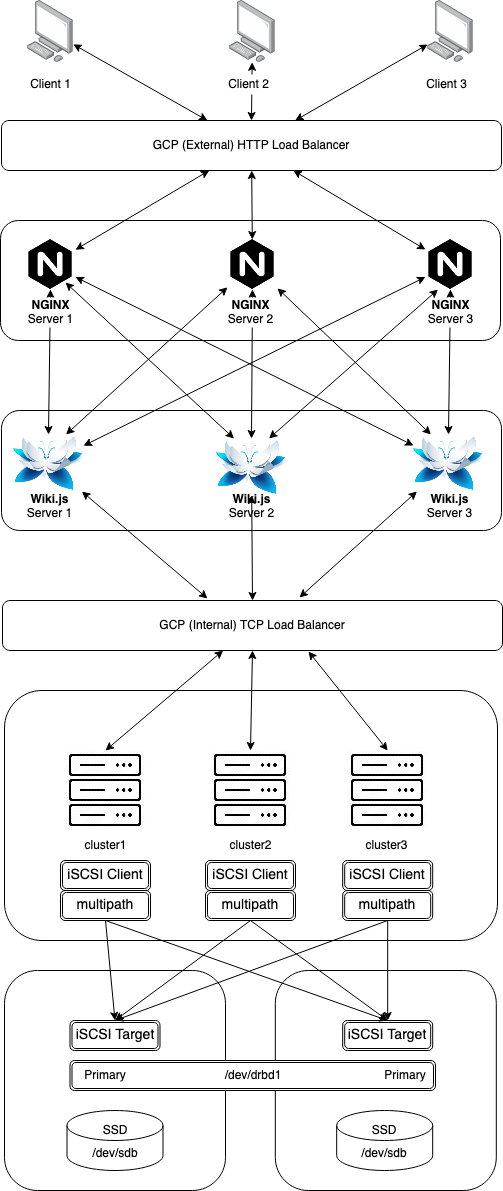
\includegraphics[width=0.54\linewidth]{img/wiki_deploy.png}
    \caption{Arquitetura Implementada}
    \label{fig:final-arch}
\end{figure}


\subsection{Testes de Carga}

Uma vez implementada a topologia apresentada na Figura \ref{fig:final-arch}, voltámos a realizar os mesmos teste de carga já referidos, mas desta vez nesta nova arquitectura de alta disponibilidade e desempenho.

\textbf{Nota:} de referir que para facilitar a leitura e suprimir a necessidade de voltar atrás para se perceber qual o objetivo dos demais testes, as descrições apresentadas acima voltam a ser apresentadas nesta secção.

\subsubsection{Teste 1}

% Inicio do Teste 1 - Diogo Monteiro - BullDogChinês

Tal como previamente descrito, o teste 1 visa representar o cenário mais básico: um utilizador aceder à página inicial da wiki. Para a realização deste teste, irão ser utilizadas mais \textit{threads} do que nos restantes, dado que num cenário real, o acesso à página inicial da wiki será a ação mais comum. O método que será testado é o seguinte:

\begin{enumerate}
  \item GET /
\end{enumerate}

O teste foi corrido com 100, 1000, 5000 e 10000 \textit{threads} (utilizadores), sendo que recorremos aos relatórios gerados pelo \textit{JMeter} para apresentar os seguintes resultados:

\begin{table}[h!]
\centering
    \begin{tabular}{ |c|c|c|c|  }
        \hline
        \multicolumn{4}{|c|}{Página Inicial} \\
        \hline
         Threads & Erro & Tempo Resposta Médio (ms) & \textit{Throughput (Trans./s)}\\
        \hline
        100   & 0.00\%   & 	89.32  & 98.81 \\
        1000  & 0.00\%   & 2929.41 & 124.64	\\
        5000  & 35.20\%  & 14183.61 & 132.07 \\
        10000 & 53.29\%  & 18069.55 & 199.77 \\
        \hline
    \end{tabular}
    \caption{Deployment - Sumário do Teste 1}
    \label{table:1}
\end{table}

Realizando uma análise aos dados da tabela, podemos, novamente, verificar que nas situações em que utilizamos 100 e 1000 utilizadores não obtemos nenhuma percentagem de erro. À medida que esses valores sobem para a casa dos 5000 já começámos a obter uma percentagem significativa de erros, sendo que com 10000 essa percentagem é ainda maior. Esta situação também se repetia na tipologia anterior, porém, em comparação, a percentagem de erros desta versão sofreu uma redução considerável em ambos os casos.

Para além disso e tal como esperado, o aumento do número de threads provocou tanto o aumento do \textit{throughput} como dos tempos médios de resposta da aplicação. Tal como no caso da percentagem de erros, comparativamente à versão anterior, ambos os valores sofreram uma \textbf{enorme} melhoria.\\
\\

\begin{figure}[ht!]
    \centering
    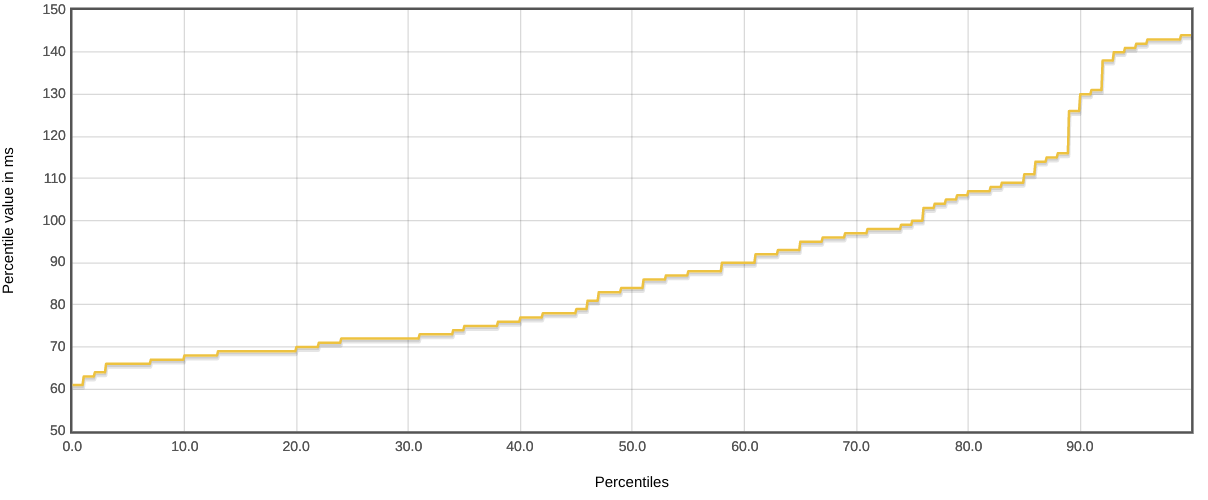
\includegraphics[width=.45\linewidth]{img/testes/i2-t1-100.png}
    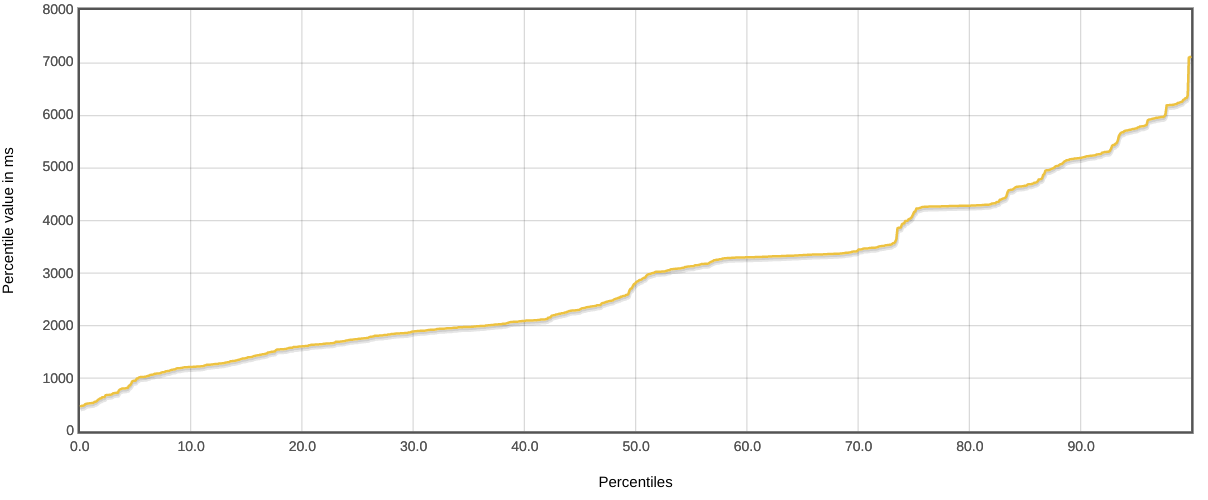
\includegraphics[width=.45\linewidth]{img/testes/i2-t1-1000.png}
    \caption{Percentil Tempo de Resposta para 100 e 1000 Threads}
\end{figure}

\begin{figure}[ht!]
    \centering
    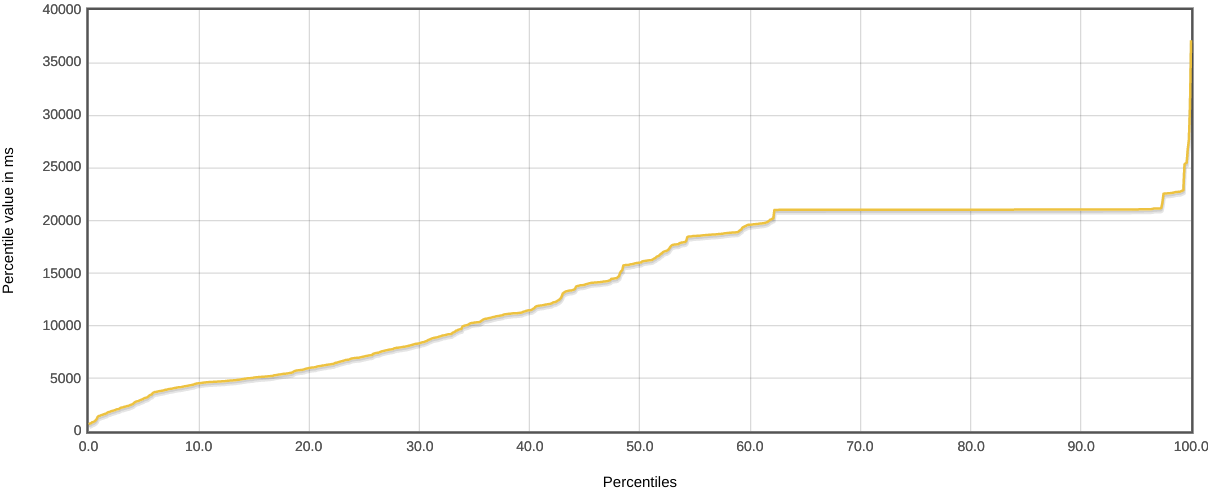
\includegraphics[width=.45\linewidth]{img/testes/i2-t1-5000.png}
    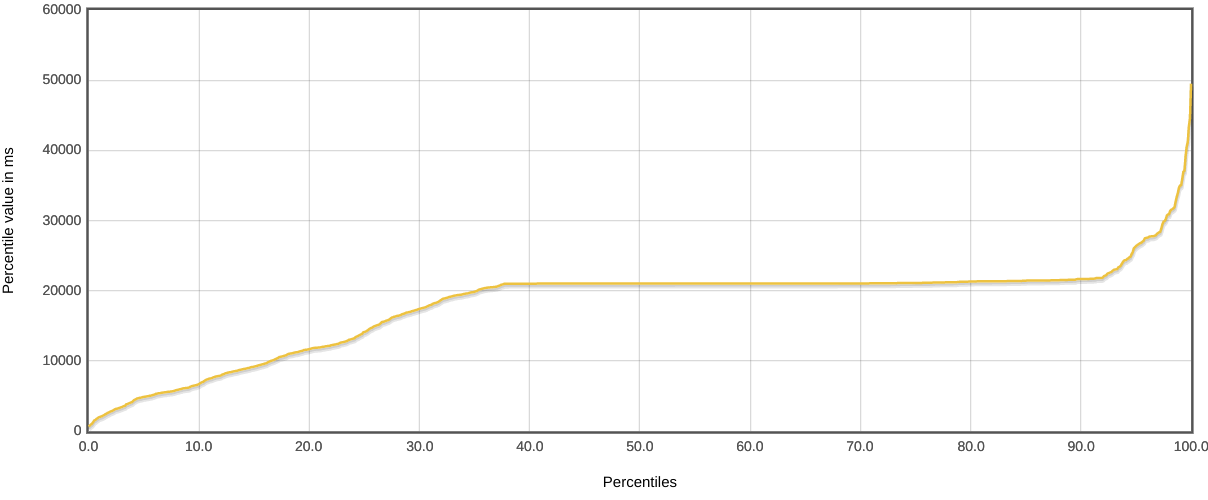
\includegraphics[width=.45\linewidth]{img/testes/i2-t1-10000.png}
    \caption{Percentil Tempo de Resposta para 5000 e 10000 Threads}
\end{figure}

Por fim, este primeiro teste veio demonstrar que contrariamente à implementação anterior, a nova arquitectura, que implementámos, é capaz de fornecer tempos de resposta perfeitamente aceitáveis, mas com uma percentagem de erro que, apesar de ter sofrido uma melhoria considerável, permanece alta.

% Fim do Teste 1 - Diogo Monteiro - BullDogChinês

\subsubsection{Teste 2}

O Teste 2 visa representar o cenário em que um utilizador entra na página inicial, navegando de seguida para uma outra página da wiki. Neste caso em específico, todas as \textit{threads} abrem a mesma página após pedirem a página inicial e esperarem 1000 milissegundos. Ao correr este teste são testados os seguintes métodos:

\begin{enumerate}
  \item GET /
  \item GET /en/ICD
\end{enumerate}

O teste foi corrido com 1000 e 5000 \textit{threads}, sendo que recorremos aos relatórios gerados pelo \textit{JMeter} para apresentar os seguintes resultados. Estes valores foram escolhidos pela sua relevância tendo em conta o teste anterior.

\begin{table}[h!]
\centering
    \begin{tabular}{ |c|c|c|c|c|  }
        \hline
        \multicolumn{4}{|c|}{Página Inicial} \\
        \hline
         Threads & Erro & Tempo Resposta Médio (ms) & \textit{Throughput (Trans./s)}\\
        \hline
        1000  & 0.00\%   & 1439.57  & 201.03\\
        5000  & 24.26\%  & 9570.59 & 226.88\\
        \hline
    \end{tabular}
    \caption{Deployment - Sumário do Teste 2}
    \label{table:1}
\end{table}

Analisando os dados da tabela, podemos verificar que com 1000 utilizadores não obtemos nenhuma percentagem de erro. Quando aumentamos para valores na casa dos 5000 começámos a obter uma percentagem significativa de erros.

Ao aumentar o número de threads, verificámos também o aumento do \textit{Throughput} da aplicação, bem como do tempo de resposta médio aos pedidos. Este último valor, dado que também serve de medida de performance do sistema, mostra-nos que nos casos em que assegurámos que todos os pedidos são atendidos, estes esperam uma quantidade de tempo considerável. 

Em relação à arquitectura inicial, podemos ver que o tempo de resposta médio diminui drasticamente para ambos os números de threads, bem como o aumento do \textit{throughput}. No entanto, este último teve valores semelhantes para número de threads diferentes, o que não acontecia anteriormente. A percentagem de erros também diminui significativamente, para metade no caso das 5000 threads. 

\begin{figure}[ht!]
    \centering
    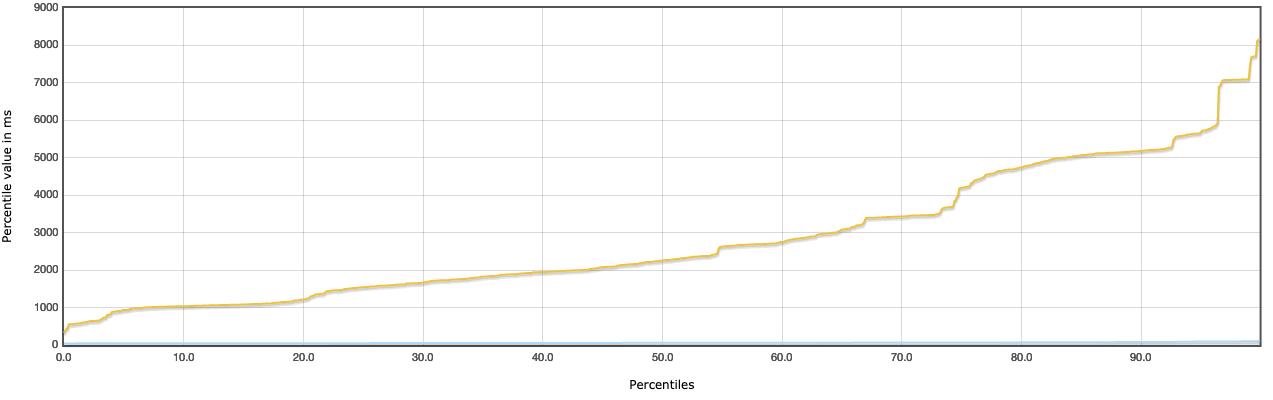
\includegraphics[width=.45\linewidth]{img/testes/i2-t2-1000.png}
    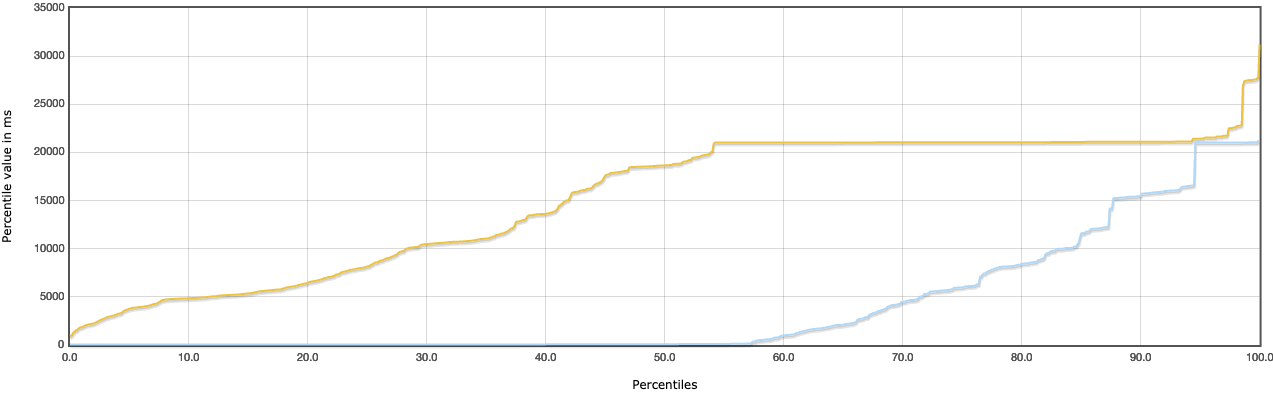
\includegraphics[width=.45\linewidth]{img/testes/i2-t2-5000.png}
    \caption{Percentil Tempo de Resposta para 1000 e 5000 Threads}
\end{figure}

Verificando os gráficos apresentados, em que a linha azul representa os pedidos referentes à página de teste e a linha laranja os pedidos referentes à página inicial. Ao contrário da arquitectura inicial, podemos ver que há agora uma grande diferença de tempos de resposta entre as duas operações.

\subsubsection{Teste 3}

O Teste 3 visa representar o cenário em que um administrador efetua login no sistema, sendo redirecionado para a página principal. Ao correr este teste são testados os seguintes métodos:

\begin{enumerate}
  \item GET  /login
  \item POST /graphql
  \item GET  /
\end{enumerate}

O teste foi corrido com 100, 250, 500, 1000 e 5000 \textit{threads}, sendo que recorremos aos relatórios gerados pelo JMeter para apresentar os seguintes resultados.
O processo de login é constituido pelos 3 pedidos apresentados, sendo que o conteúdo do POST que é feito possui o endereço de email e a password da conta utilizada no teste. Estes 3 pedidos foram encapsulados num processo mais generalizado que representa o login como um todo. Optámos por esta visão de modo a representar de modo mais fidedigno o ato de efetuar login, dado que não é possível efetuar login se uma das operações falhar. Outra atenção que tivemos, foi o cancelamento de uma \textit{thread} no caso de um dos pedidos falhar.

\begin{table}[h!]
\centering
    \begin{tabular}{ |c|c|c|c|c|  }
        \hline
        \multicolumn{4}{|c|}{Página Inicial} \\
        \hline
         Threads & Erro & Tempo Resposta Médio (ms) & \textit{Throughput (Trans./s)}\\
        \hline
        100   & 0.00\%   & 1987.23  & 39.48\\
        250   & 0.00\%   & 2397.48  & 83.31\\
        500   & 0.00\%   & 2951.27 & 124.53\\
        1000  & 0.00\%   & 3185.77 & 120.18\\
        5000  & 25.78\%  & 12737.36 & 95.51\\
        \hline
    \end{tabular}
    \caption{Deployment - Sumário do Teste 3}
    \label{table:1}
\end{table}

Analisando os dados da tabela, podemos verificar que com 100, 250, 500 e 1000 não obtemos nenhuma percentagem de erro. Ao aumentar o número de threads, verificámos também o aumento do \textit{Throughput} da aplicação até um certo ponto, sendo que começou a diminuir a partir das 1000 threads. O tempo de resposta médio aos pedidos por sua vez não estagnou, subindo para valores elevados, mesmo sem a ocorrência de erros.

Em relação à arquitectura inicial, podemos ver que o tempo de resposta médio diminui drasticamente para todas as threads, bem como o aumento do \textit{throughput}, apesar deste começar a diminuir a certo ponto. Isto significa que a partir de um dado ponto a performance se começa a degradar acentuadamente. Quanto à percentagem de erros conseguimos eliminar por completo no caso das 1000 threads enquanto que na de 5000 obtemos resultados 2.5 vezes melhores. 

Nos gráficos apresentados, as \textbf{linhas vermelhas} representam o pedido \textbf{GET /login}, as \textbf{linhas azuis} representam o pedido \textbf{POST /graphql}, as \textbf{linhas amarelas} representam o pedido \textbf{GET /} e as \textbf{linhas verdes} representam o \textbf{Login} como um todo.


\begin{figure}[ht!]
    \centering
    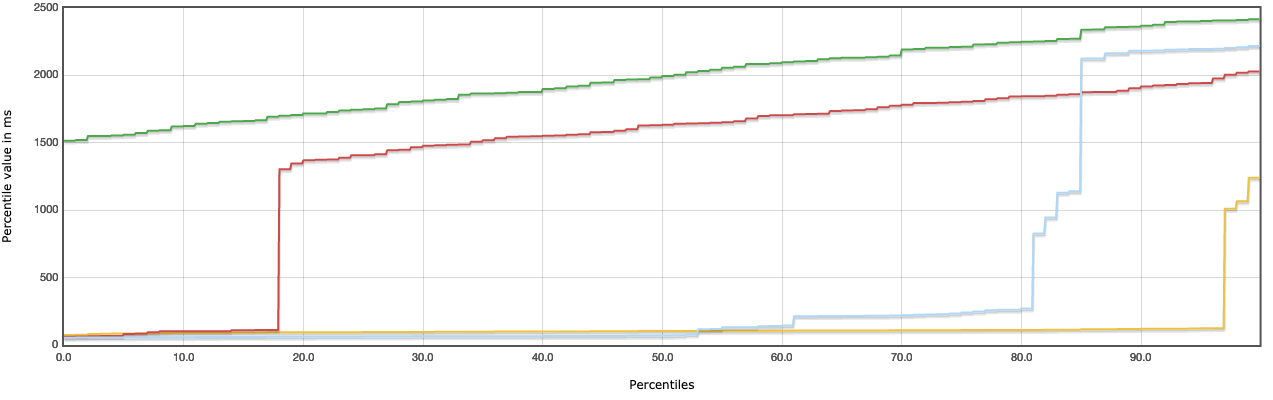
\includegraphics[width=.45\linewidth]{img/testes/i2-t3-100.png}
    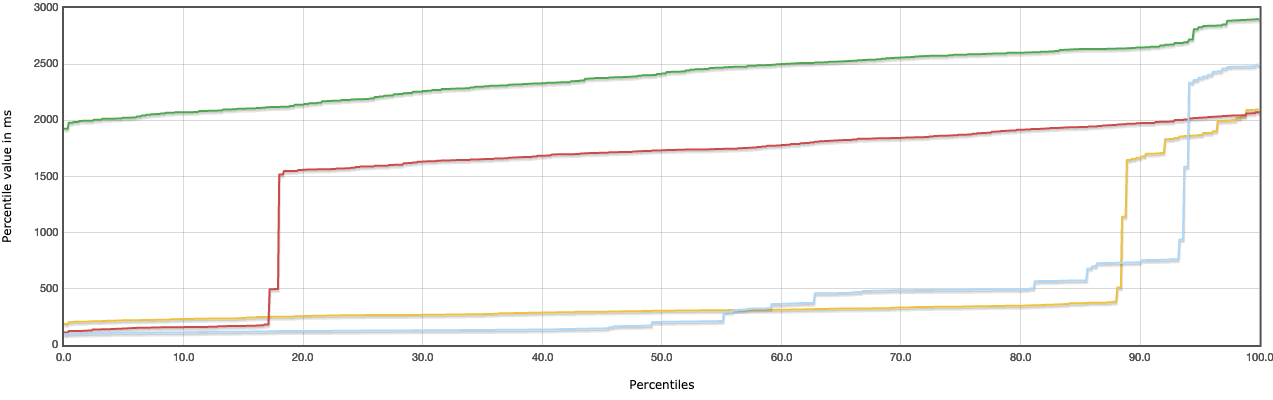
\includegraphics[width=.45\linewidth]{img/testes/i2-t3-250.png}
    \caption{Percentil Tempo de Resposta para 100 e 250 Threads}
\end{figure}

\begin{figure}[ht!]
    \centering
    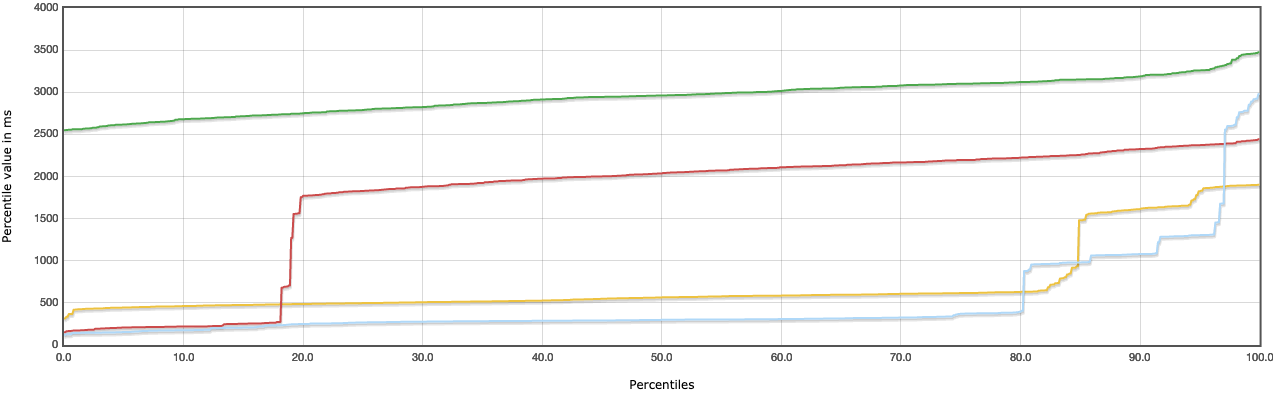
\includegraphics[width=.45\linewidth]{img/testes/i2-t3-500.png}
    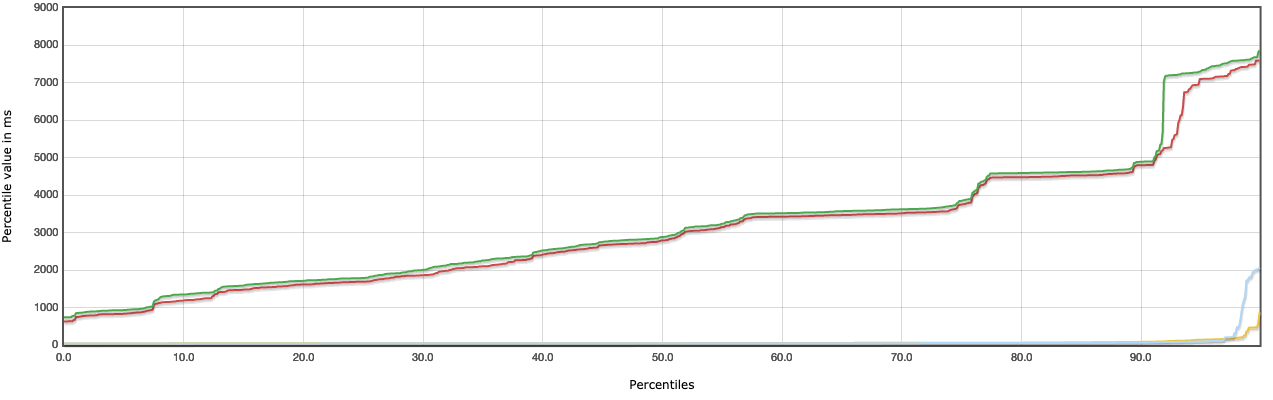
\includegraphics[width=.45\linewidth]{img/testes/i2-t3-1000.png}
    \caption{Percentil Tempo de Resposta para 500 e 1000 Threads}
\end{figure}

\begin{figure}[ht!]
    \centering
    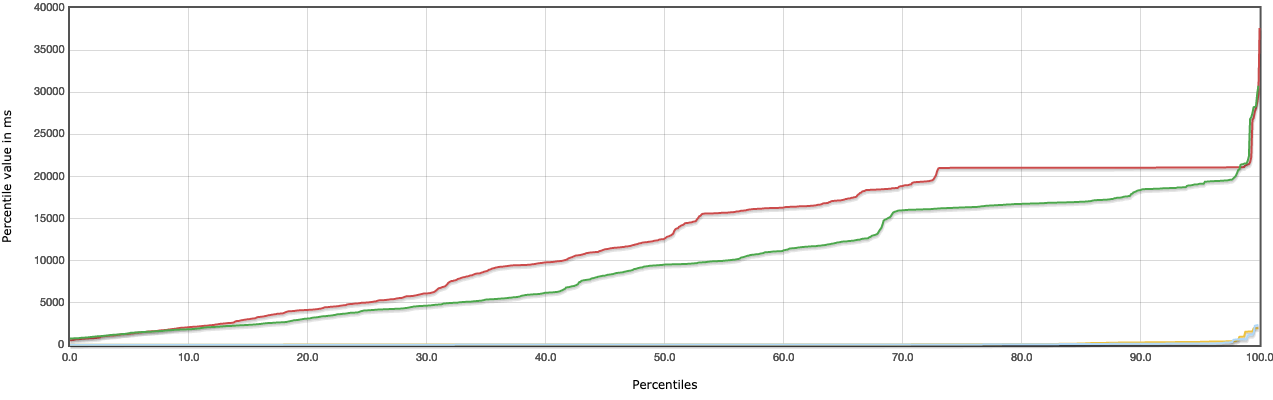
\includegraphics[width=.9\linewidth]{img/testes/i2-t3-5000.png}
    \caption{Percentil Tempo de Resposta para 5000 Threads}
\end{figure}

Ao contrário da arquitectura inicial, podemos ver que há agora uma grande diferença de tempos de resposta entre as operações. Anteriormente todas elas tinham a sua relevância enquanto que agora apenas as operações de LOGIN e GET LOGIN são comparativamente mais demoradas.

\subsubsection{Teste 4}

% Inicio do Teste 4 - Diogo Monteiro - BullDogChinês

O Teste 4 visa representar o cenário em que um administrador efetua login no sistema, sendo redireccionado para a página principal, seguido da criação de uma nova página wiki. Este teste irá testar os seguintes métodos:

\begin{enumerate}
    \item GET /login
    \item POST /graphql
    \item GET /
    \item GET /e/en/ThreadNum-Pagename
    \item POST /graphql
    \item GET /e/en/ThreadNum-Pagename
\end{enumerate}

Tal como explicado acima, nos métodos podemos encontrar as palavras \textit{ThreadNum} e \textit{Pagename}, que na verdade são variáveis. Cada \textit{thread} onde corremos os testes terá um \textit{ThreadNum} único, de maneira a conseguirmos saber que páginas cada \textit{thread} criou, e optamos por dar o nome à página a data do momento em que é criada em milissegundos para sabermos quando e por que ordem foram criadas as novas páginas. Isto é possível tomando partido das funções \texttt{\_\_time()} e \texttt{\_\_threadNum} do \textit{JMeter}.

O teste foi corrido com 100, 250 e 500 \textit{threads}, sendo que recorremos aos relatórios gerados pelo \textit{JMeter} para apresentar os seguintes resultados. A única diferença entre este teste e o anterior é que agora criamos uma página nova depois de fazermos o login, enquanto que no outro o teste acabaria precisamente depois de realizarmos o login. O processo de criação duma nova página é constituído pelos 3 últimos pedidos apresentados, sendo que o conteúdo do POST possui o conteúdo que a nova página irá apresentar. Estes 3 pedidos foram encapsulados num processo mais generalizado que representa a criação duma nova página como um todo. Optámos por esta visão de modo a representar de modo mais fidedigno o ato de criar uma nova página, dado que não é possível criá-la se uma das operações falhar. Sendo assim, preferimos separar a operação de efetuar login da criação da nova página para podermos avaliar individualmente cada um dos processos. 

\begin{table}[H]
\centering
\begin{tabular}{|c|c|c|p{3.5cm}|p{3cm}|}
\hline
Threads              & Operação & Erro    & Tempo Resposta Médio (ms) & \textit{Throughput (Trans./s)} \\ \hline
\multirow{2}{*}{100} & Login    & 0.00\%  & 3705.34                   & 37.645                          \\
                     & New Page & 0.00\% & 84141.29                 & 4,31                           \\ \hline
\multirow{2}{*}{250} & Login    & 0.00\%  & 3997.54                  & 46.75                          \\
                     & New Page & 0.00\% & 161938.23                 & 2.32                           \\ \hline
\multirow{2}{*}{500} & Login    & 0.00\%  & 6516.45                  & 17.14                         \\
                     & New Page & 0.00\% & 306854.25                 & 1.7                          \\ \hline
\end{tabular}
\caption{Deployment - Sumário do Teste 4}
\end{table}

Realizando uma análise aos dados recolhidos, podemos verificar que as operações de login continuam a ser realizadas sem qualquer erro. Porém, contrariamente à percentagem de erros que a versão anterior evidenciava, esta nova topologia reduz essa percentagem para 0 em todas as situações. Para além disto, esta nova versão apresenta uma estagnação quando o número de utilizadores cresce, começando a haver uma degradação nos tempos de resposta e começando o \textit{throughput} a cair. Isto leva-nos a crer que estamos a lidar com um número de utilizadores já acima da capacidade do sistema, começando os valores a ser pouco fidedignos.

Nos gráficos apresentados, as linhas \textbf{vermelho-escuro, roxo e amarelo-escuro} são as mais visíveis e ao mesmo tempo preocupantes, representando o \textbf{login, New Page e GET Page}, respetivamente.
\pagebreak

\begin{figure}[ht!]
    \centering
    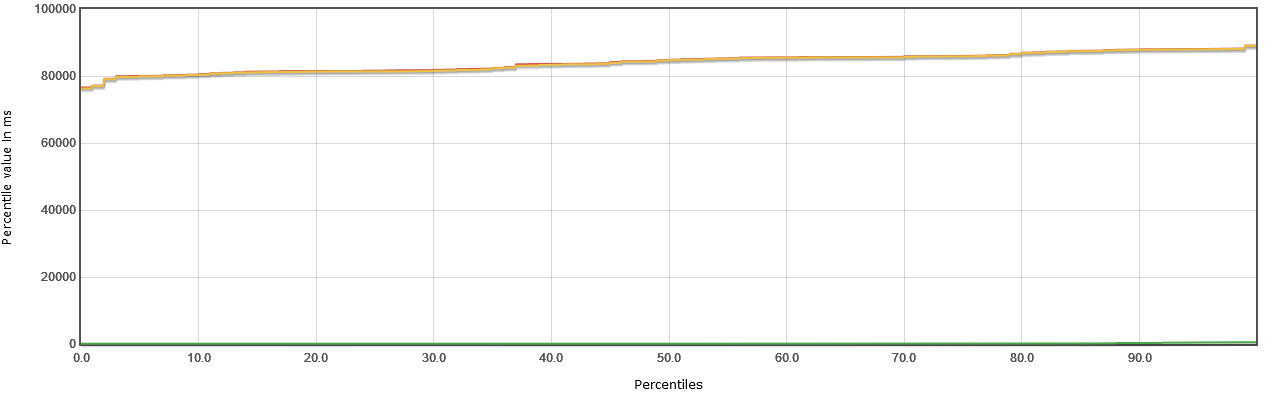
\includegraphics[width=.85\linewidth]{img/testes/i2-t4-100.png}
    \caption{Percentil Tempo de Resposta para 100 Threads}
\end{figure}

\begin{figure}[ht!]
    \centering
    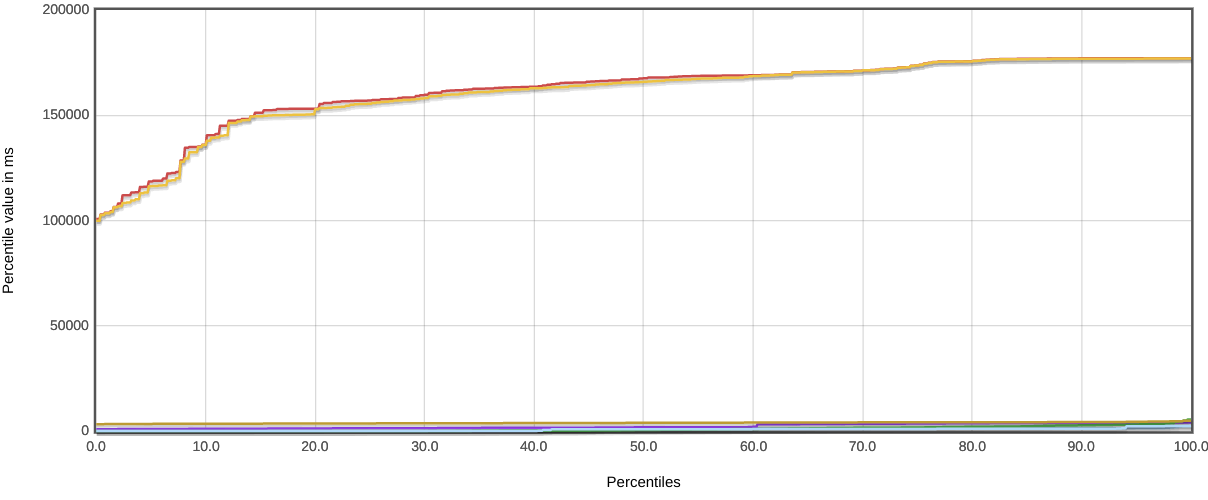
\includegraphics[width=.85\linewidth]{img/testes/i2-t4-250.png}
    \caption{Percentil Tempo de Resposta para 250 Threads}
\end{figure}

\begin{figure}[ht!]
    \centering
    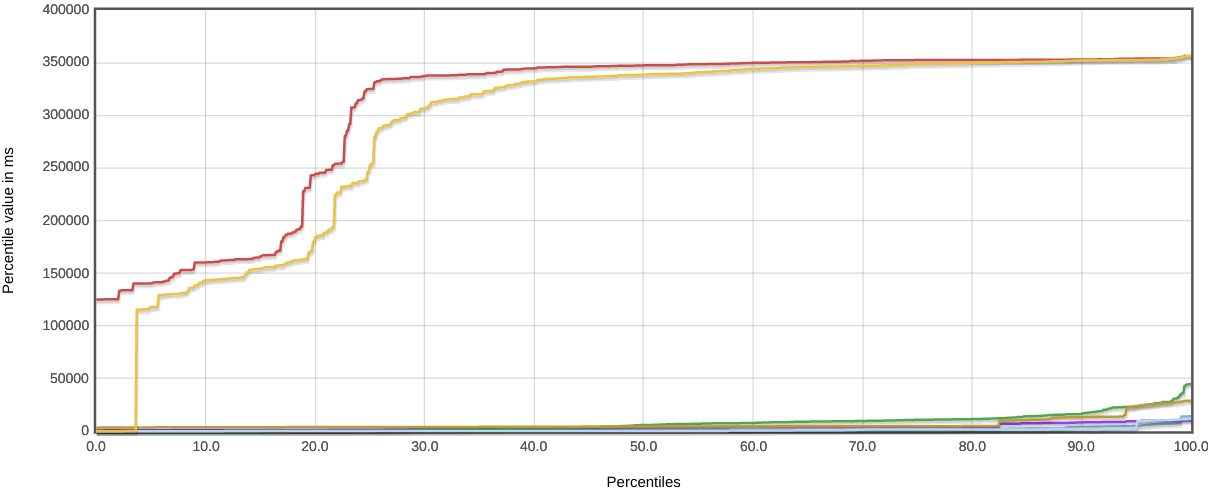
\includegraphics[width=.85\linewidth]{img/testes/i2-t4-500.png}
    \caption{Percentil Tempo de Resposta para 500 Threads}
\end{figure}

Em conclusão, no que diz respeito ao teste 4, esta nova topologia demonstra um excelente redução da percentagem de erro para a criação de uma nova página, mostrando assim uma melhoria na disponibilidade da plataforma. No entanto existem alguns aspetos a melhorar, nomeadamente a nível de performance, dado que gostaríamos de melhorar um pouco os tempos de resposta.

% VOLTAR A REVER O TESTE PARA AS 100 THREADS

% 100 THREADS ESTÁ MAL

% Fim do Teste 4 - Diogo Monteiro - BullDogChinês

\subsection{Análise de Desempenho}

% Não finalizado

Neste ponto, tendo uma arquitectura distribuída, é de esperar um aumento de disponibilidade e performance da aplicação, como foi mostrado anteriormente através da comparação dos resultados dos testes de carga das arquiteturas Inicial e Final. No entanto, apenas as camadas aplicacionais e web correm paralelamente, o que explica que as melhorias mais significativas sejam em pedidos menos dependentes da base de dados. Dado que o principal foco foi a disponibilidade do sistema, a principal alteração na camada de persistência foi a replicação do armazenamento. Isto apenas nos fornece redundância dos dados, não garantindo melhorias de performance em operações na base de dados. 

Olhando para o nosso principal objetivo, garantir elevada disponibilidade, podemos dizer que obtivemos sucesso, dado que todas as operações com uma percentagem de erro não nula diminuíram consideravelmente, e dado que o sistema é capaz de resistir a falhas de componentes. A nível de performance, os nossos testes de carga revelam que também obtivemos melhorias significativas, especialmente devido ao balanceamento de carga por parte das camadas \textit{web} e aplicacional.

\subsection{Mitigação dos Pontos Críticos do Sistema}

Após a implementação da plataforma e execução de testes de carga, podemos avaliar os pontos críticos identificados na secção 3.1.

Um dos pontos críticos identificados foi a possibilidade de uma ou mais componentes do sistema falharem, causando uma interrupção do serviço. Esse problema foi mitigado, dado que os dados se encontram replicados e nenhuma componente do sistema possui uma só instância.

Foram também mencionados pontos críticos no sistema sob a forma de \textit{bottlenecks}, tendo estes tendo sido maioritariamente mitigados. A nível dos servidores aplicacionais e \textit{web}, com o uso de um balanceador de carga, eliminámos o \textit{bottleneck} por completo. No entanto, na nossa base de dados, apesar das melhorias de performance, esta continua em parte a ser um \textit{bottleneck} do sistema, dado que as operações mais lentas estão diretamente relacionadas com pedidos feitos à mesma. A conclusão a que chegámos é que para melhorar a performance do sistema como um todo, a implementação da base de dados terá de ser diferente. Como o nosso principal foco é a disponibilidade, optámos por manter a nossa arquitetura dado que satisfaz os nossos requisitos. 

Apesar de resolver uma boa parte dos problemas existentes, existem alguns quer irão sempre persistir, e que por muito improváveis que possam ou não ser, devem ser considerados. Apesar de termos todas as componentes replicadas, se falharem os 3 nós do cluster de armazenamento em simultâneo, o nosso sistema irá falhar. O mesmo se aplica aos servidores NGINX e aos servidores Wiki.js, bem como às duas instâncias que compõem o drbd. Outro problema que poderá existir é o caso de um dos \textit{load balancers} falhar, tornando o nosso sistema inoperacional.

Resumindo, no caso de todas as instâncias de uma das camadas falharem ou de um dos \textit{load balancers} falhar, o nosso sistema ficará indisponível, apesar de se tratarem de situações improváveis. 

Visto isto, podemos afirmar que a arquitetura implementada garante elevada disponibilidade.

\pagebreak
\section{Conclusions}
From what was possible to understand from this study, it can be concluded that when we are dealing with a market research study, consumers' input and opinion is crucial to accurately grasp and understand the importance of multiple factors and their relationships in the respective market.

Furthermore, considering the model described in section \ref{section:model} and its respective results, detailed in section \ref{section:results}, it is clear that, despite the current limited capabilities of the underlying technology and the restricted technological evolution of Electric Vehicles, the growth of the EV market, regarding its population of adopters has an exponential behaviour, leading to the belief that, at some point in the future, the personal vehicles market will be dominated by EVs.

Moreover, it also reasonable to conclude that a major factor to help accelerate the purchase of EVs and promote its further development is the government subsidies, being the price one of the greatest obstacles to consumers when considering to buy an EV. The other obstacle to current EV adoption is the driving range of these vehicles, that is quite limited in current models, however, the implementation of a well distributed recharging infrastructure with optimal coverage is key to minimize this factor and mitigate the existent doubt of transportation viability with an EV.

\clearpage
\appendix
\section{Wiki.js - configuração simples com Docker Compose}\label{appendix:wiki-docker-compose}
\begin{lstlisting}[language=docker-compose-2]
version: "3.8"
services:
  db:
    image: postgres:alpine
    environment:
      POSTGRES_DB: wiki
      POSTGRES_PASSWORD: wikijsrocks
      POSTGRES_USER: wikijs
    logging:
      driver: "none"
    restart: unless-stopped
    volumes:
      - db-data:/var/lib/postgresql/data

  wiki:
    image: requarks/wiki:2
    depends_on:
      - db
    environment:
      DB_TYPE: postgres
      DB_HOST: db
      DB_PORT: 5432
      DB_USER: wikijs
      DB_PASS: wikijsrocks
      DB_NAME: wiki
    restart: unless-stopped
    ports:
      - "80:3000"

volumes:
  db-data:
\end{lstlisting}
\clearpage


%prints bibliography from bibliography file.
\printbibliography

\end{document}
